\documentclass[1p]{elsarticle_modified}
%\bibliographystyle{elsarticle-num}

%\usepackage[colorlinks]{hyperref}
%\usepackage{abbrmath_seonhwa} %\Abb, \Ascr, \Acal ,\Abf, \Afrak
\usepackage{amsfonts}
\usepackage{amssymb}
\usepackage{amsmath}
\usepackage{amsthm}
\usepackage{scalefnt}
\usepackage{amsbsy}
\usepackage{kotex}
\usepackage{caption}
\usepackage{subfig}
\usepackage{color}
\usepackage{graphicx}
\usepackage{xcolor} %% white, black, red, green, blue, cyan, magenta, yellow
\usepackage{float}
\usepackage{setspace}
\usepackage{hyperref}

\usepackage{tikz}
\usetikzlibrary{arrows}

\usepackage{multirow}
\usepackage{array} % fixed length table
\usepackage{hhline}

%%%%%%%%%%%%%%%%%%%%%
\makeatletter
\renewcommand*\env@matrix[1][\arraystretch]{%
	\edef\arraystretch{#1}%
	\hskip -\arraycolsep
	\let\@ifnextchar\new@ifnextchar
	\array{*\c@MaxMatrixCols c}}
\makeatother %https://tex.stackexchange.com/questions/14071/how-can-i-increase-the-line-spacing-in-a-matrix
%%%%%%%%%%%%%%%

\usepackage[normalem]{ulem}

\newcommand{\msout}[1]{\ifmmode\text{\sout{\ensuremath{#1}}}\else\sout{#1}\fi}
%SOURCE: \msout is \stkout macro in https://tex.stackexchange.com/questions/20609/strikeout-in-math-mode

\newcommand{\cancel}[1]{
	\ifmmode
	{\color{red}\msout{#1}}
	\else
	{\color{red}\sout{#1}}
	\fi
}

\newcommand{\add}[1]{
	{\color{blue}\uwave{#1}}
}

\newcommand{\replace}[2]{
	\ifmmode
	{\color{red}\msout{#1}}{\color{blue}\uwave{#2}}
	\else
	{\color{red}\sout{#1}}{\color{blue}\uwave{#2}}
	\fi
}

\newcommand{\Sol}{\mathcal{S}} %segment
\newcommand{\D}{D} %diagram
\newcommand{\A}{\mathcal{A}} %arc


%%%%%%%%%%%%%%%%%%%%%%%%%%%%%5 test

\def\sl{\operatorname{\textup{SL}}(2,\Cbb)}
\def\psl{\operatorname{\textup{PSL}}(2,\Cbb)}
\def\quan{\mkern 1mu \triangleright \mkern 1mu}

\theoremstyle{definition}
\newtheorem{thm}{Theorem}[section]
\newtheorem{prop}[thm]{Proposition}
\newtheorem{lem}[thm]{Lemma}
\newtheorem{ques}[thm]{Question}
\newtheorem{cor}[thm]{Corollary}
\newtheorem{defn}[thm]{Definition}
\newtheorem{exam}[thm]{Example}
\newtheorem{rmk}[thm]{Remark}
\newtheorem{alg}[thm]{Algorithm}

\newcommand{\I}{\sqrt{-1}}
\begin{document}

%\begin{frontmatter}
%
%\title{Boundary parabolic representations of knots up to 8 crossings}
%
%%% Group authors per affiliation:
%\author{Yunhi Cho} 
%\address{Department of Mathematics, University of Seoul, Seoul, Korea}
%\ead{yhcho@uos.ac.kr}
%
%
%\author{Seonhwa Kim} %\fnref{s_kim}}
%\address{Center for Geometry and Physics, Institute for Basic Science, Pohang, 37673, Korea}
%\ead{ryeona17@ibs.re.kr}
%
%\author{Hyuk Kim}
%\address{Department of Mathematical Sciences, Seoul National University, Seoul 08826, Korea}
%\ead{hyukkim@snu.ac.kr}
%
%\author{Seokbeom Yoon}
%\address{Department of Mathematical Sciences, Seoul National University, Seoul, 08826,  Korea}
%\ead{sbyoon15@snu.ac.kr}
%
%\begin{abstract}
%We find all boundary parabolic representation of knots up to 8 crossings.
%
%\end{abstract}
%\begin{keyword}
%    \MSC[2010] 57M25 
%\end{keyword}
%
%\end{frontmatter}

%\linenumbers
%\tableofcontents
%
\newcommand\colored[1]{\textcolor{white}{\rule[-0.35ex]{0.8em}{1.4ex}}\kern-0.8em\color{red} #1}%
%\newcommand\colored[1]{\textcolor{white}{ #1}\kern-2.17ex	\textcolor{white}{ #1}\kern-1.81ex	\textcolor{white}{ #1}\kern-2.15ex\color{red}#1	}

{\Large $\underline{12a_{0033}~(K12a_{0033})}$}

\setlength{\tabcolsep}{10pt}
\renewcommand{\arraystretch}{1.6}
\vspace{1cm}\begin{tabular}{m{100pt}>{\centering\arraybackslash}m{274pt}}
\multirow{5}{120pt}{
	\centering
	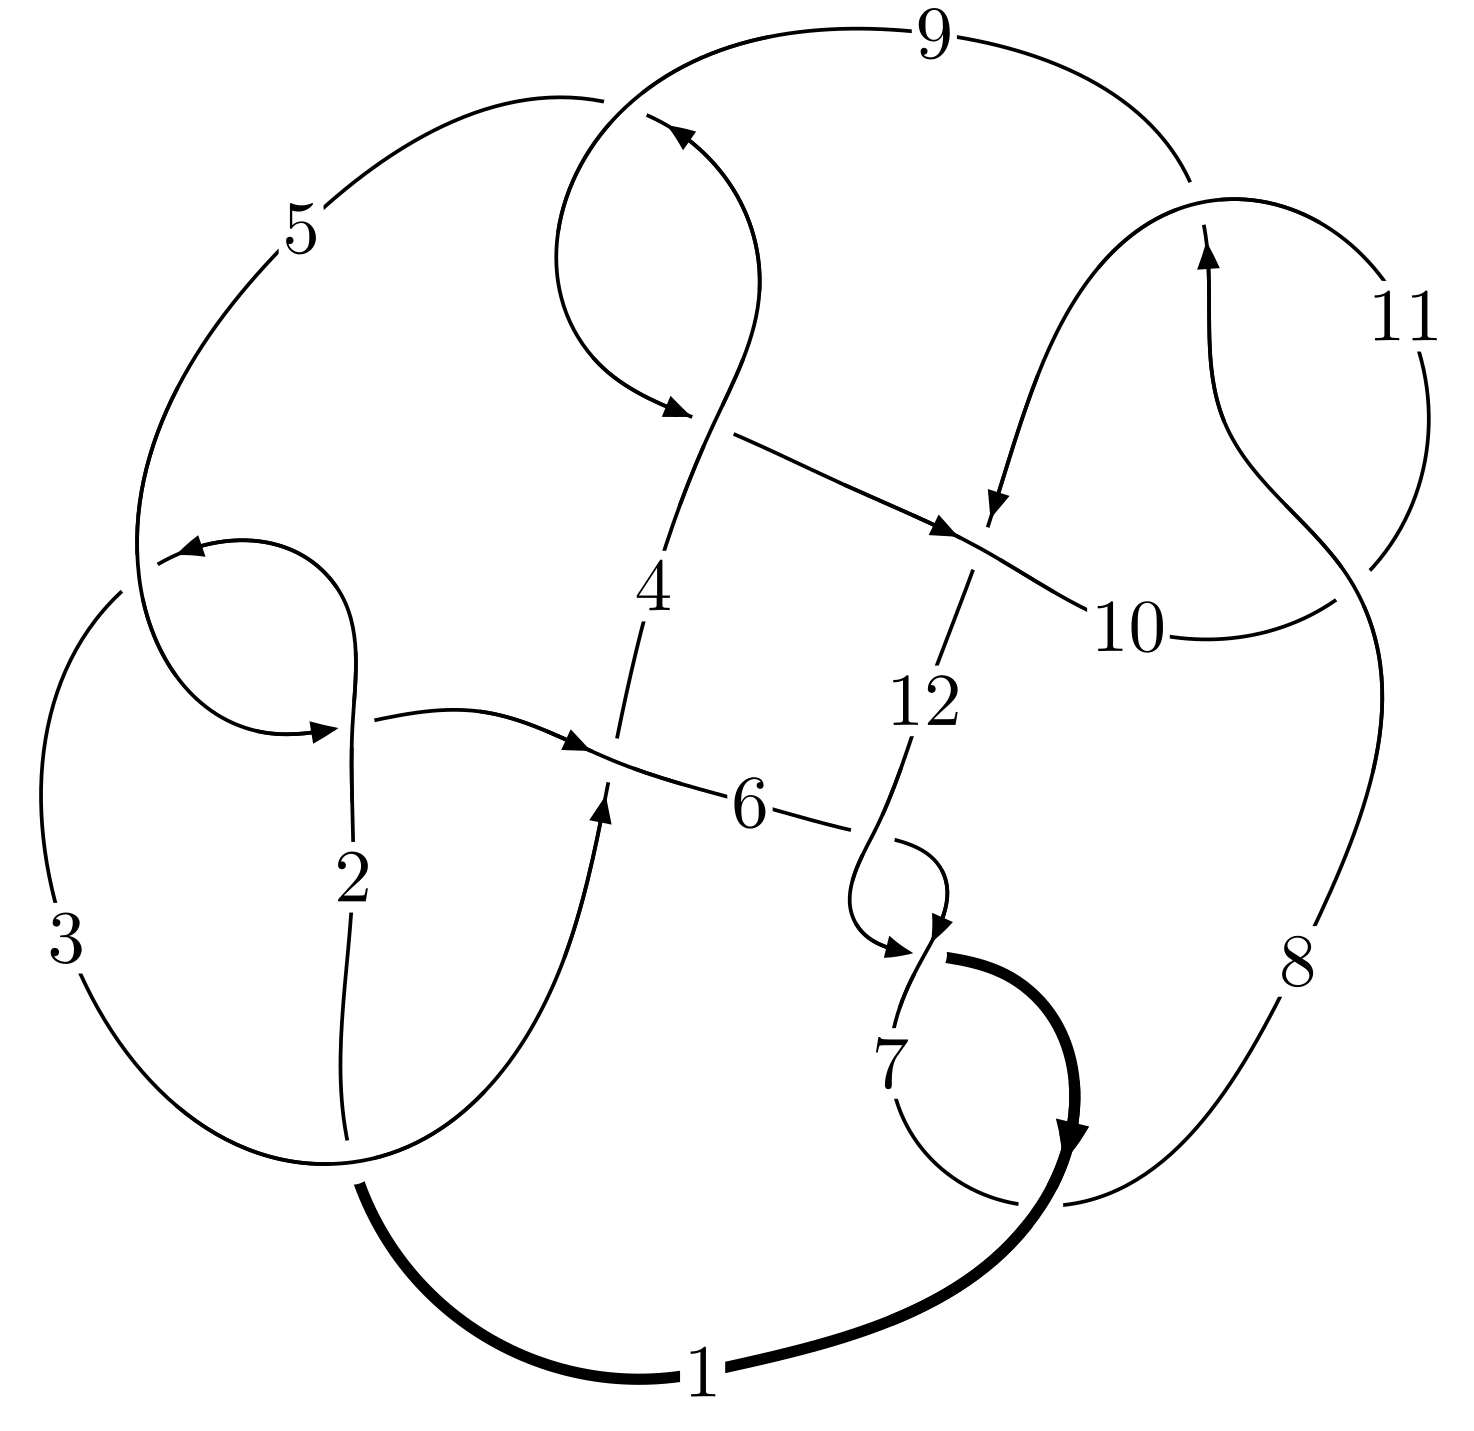
\includegraphics[width=112pt]{../../../GIT/diagram.site/diagram/png/834_12a_0033.png}\\
\ \ \ A knot diagram\footnotemark}&
\allowdisplaybreaks
\textbf{Linearized knot diagam} \\
\cline{2-2}
 &
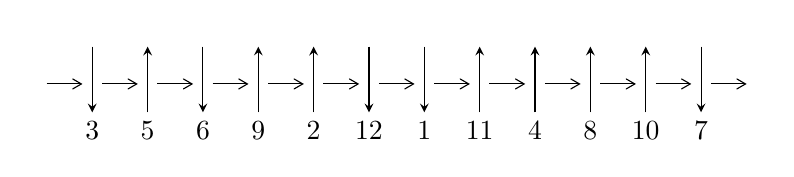
\begin{tikzpicture}[x=20pt, y=17pt]
	% nodes
	\node (C0) at (0, 0) {};
	\node (C1) at (1, 0) {};
	\node (C1U) at (1, +1) {};
	\node (C1D) at (1, -1) {3};

	\node (C2) at (2, 0) {};
	\node (C2U) at (2, +1) {};
	\node (C2D) at (2, -1) {5};

	\node (C3) at (3, 0) {};
	\node (C3U) at (3, +1) {};
	\node (C3D) at (3, -1) {6};

	\node (C4) at (4, 0) {};
	\node (C4U) at (4, +1) {};
	\node (C4D) at (4, -1) {9};

	\node (C5) at (5, 0) {};
	\node (C5U) at (5, +1) {};
	\node (C5D) at (5, -1) {2};

	\node (C6) at (6, 0) {};
	\node (C6U) at (6, +1) {};
	\node (C6D) at (6, -1) {12};

	\node (C7) at (7, 0) {};
	\node (C7U) at (7, +1) {};
	\node (C7D) at (7, -1) {1};

	\node (C8) at (8, 0) {};
	\node (C8U) at (8, +1) {};
	\node (C8D) at (8, -1) {11};

	\node (C9) at (9, 0) {};
	\node (C9U) at (9, +1) {};
	\node (C9D) at (9, -1) {4};

	\node (C10) at (10, 0) {};
	\node (C10U) at (10, +1) {};
	\node (C10D) at (10, -1) {8};

	\node (C11) at (11, 0) {};
	\node (C11U) at (11, +1) {};
	\node (C11D) at (11, -1) {10};

	\node (C12) at (12, 0) {};
	\node (C12U) at (12, +1) {};
	\node (C12D) at (12, -1) {7};
	\node (C13) at (13, 0) {};

	% arrows
	\draw[->,>={angle 60}]
	(C0) edge (C1) (C1) edge (C2) (C2) edge (C3) (C3) edge (C4) (C4) edge (C5) (C5) edge (C6) (C6) edge (C7) (C7) edge (C8) (C8) edge (C9) (C9) edge (C10) (C10) edge (C11) (C11) edge (C12) (C12) edge (C13) ;	\draw[->,>=stealth]
	(C1U) edge (C1D) (C2D) edge (C2U) (C3U) edge (C3D) (C4D) edge (C4U) (C5D) edge (C5U) (C6U) edge (C6D) (C7U) edge (C7D) (C8D) edge (C8U) (C9D) edge (C9U) (C10D) edge (C10U) (C11D) edge (C11U) (C12U) edge (C12D) ;
	\end{tikzpicture} \\
\hhline{~~} \\& 
\textbf{Solving Sequence} \\ \cline{2-2} 
 &
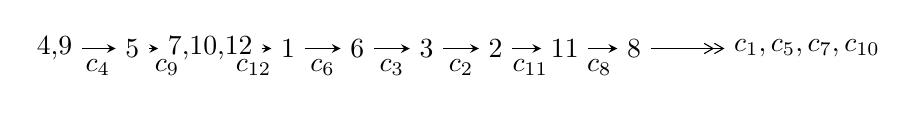
\begin{tikzpicture}[x=25pt, y=7pt]
	% node
	\node (A0) at (-1/8, 0) {4,9};
	\node (A1) at (1, 0) {5};
	\node (A2) at (17/8, 0) {7,10,12};
	\node (A3) at (13/4, 0) {1};
	\node (A4) at (17/4, 0) {6};
	\node (A5) at (21/4, 0) {3};
	\node (A6) at (25/4, 0) {2};
	\node (A7) at (29/4, 0) {11};
	\node (A8) at (33/4, 0) {8};
	\node (C1) at (1/2, -1) {$c_{4}$};
	\node (C2) at (3/2, -1) {$c_{9}$};
	\node (C3) at (11/4, -1) {$c_{12}$};
	\node (C4) at (15/4, -1) {$c_{6}$};
	\node (C5) at (19/4, -1) {$c_{3}$};
	\node (C6) at (23/4, -1) {$c_{2}$};
	\node (C7) at (27/4, -1) {$c_{11}$};
	\node (C8) at (31/4, -1) {$c_{8}$};
	\node (A9) at (43/4, 0) {$c_{1},c_{5},c_{7},c_{10}$};

	% edge
	\draw[->,>=stealth]	
	(A0) edge (A1) (A1) edge (A2) (A2) edge (A3) (A3) edge (A4) (A4) edge (A5) (A5) edge (A6) (A6) edge (A7) (A7) edge (A8) ;
	\draw[->>,>={angle 60}]	
	(A8) edge (A9);
\end{tikzpicture} \\ 

\end{tabular} \\

\footnotetext{
The image of knot diagram is generated by the software ``\textbf{Draw programme}" developed by Andrew Bartholomew(\url{http://www.layer8.co.uk/maths/draw/index.htm\#Running-draw}), where we modified some parts for our purpose(\url{https://github.com/CATsTAILs/LinksPainter}).
}\phantom \\ \newline 
\centering \textbf{Ideals for irreducible components\footnotemark of $X_{\text{par}}$} 
 
\begin{align*}
I^u_{1}&=\langle 
4.19179\times10^{162} u^{76}-8.99312\times10^{162} u^{75}+\cdots+5.13128\times10^{164} d+1.74805\times10^{165},\\
\phantom{I^u_{1}}&\phantom{= \langle  }5.20225\times10^{162} u^{76}-1.09357\times10^{163} u^{75}+\cdots+5.13128\times10^{164} c+2.30253\times10^{165},\\
\phantom{I^u_{1}}&\phantom{= \langle  }5.03182\times10^{182} u^{76}-1.22724\times10^{183} u^{75}+\cdots+1.08760\times10^{185} b+3.35895\times10^{185},\\
\phantom{I^u_{1}}&\phantom{= \langle  }-3.61857\times10^{182} u^{76}+6.18392\times10^{182} u^{75}+\cdots+5.43799\times10^{184} a-1.83798\times10^{184},\\
\phantom{I^u_{1}}&\phantom{= \langle  }u^{77}-2 u^{76}+\cdots-2560 u^2-512\rangle \\
I^u_{2}&=\langle 
-43 u^3 a^2-6 a^2 u^2-37 u^3 a-62 a^2 u-58 u^2 a+38 u^3+36 a^2-55 a u+2 u^2+71 d-78 a-74 u-12,\\
\phantom{I^u_{2}}&\phantom{= \langle  }-47 u^3 a^2+5 a^2 u^2-52 u^3 a-43 a^2 u-70 u^2 a-8 u^3+41 a^2-37 a u+22 u^2+71 c-6 a-104 u+10,\\
\phantom{I^u_{2}}&\phantom{= \langle  }-24 u^3 a^2-5 a^2 u^2-19 u^3 a-28 a^2 u- u^2 a+8 u^3+30 a^2-34 a u-22 u^2+71 b-65 a-38 u-10,\\
\phantom{I^u_{2}}&\phantom{= \langle  }-2 u^3 a^2- u^3 a+a^3-2 a^2 u-5 u^2 a- u^3+2 a^2- a u+u^2- u,\;u^4+u^2- u+1\rangle \\
I^u_{3}&=\langle 
-75 u^5 a^2+125 u^5 a+\cdots-31 a+44,\;-55 u^5 a^2+167 u^5 a+\cdots+143 a-28,\\
\phantom{I^u_{3}}&\phantom{= \langle  }-58 u^5 a^2+59 u^5 a+\cdots-30 a+28,\\
\phantom{I^u_{3}}&\phantom{= \langle  }-2 u^5 a^2-2 u^4 a^2+2 u^5 a-4 u^3 a^2+u^4 a+u^5-4 a^2 u^2+3 u^3 a+a^3-4 a^2 u-2 u^2 a-4 a^2+2 a u+2 a,\\
\phantom{I^u_{3}}&\phantom{= \langle  }u^6+u^5+2 u^4+2 u^3+2 u^2+2 u+1\rangle \\
\\
I^v_{1}&=\langle 
a,\;d- v+1,\;c+a,\;b+v-1,\;v^2- v+1\rangle \\
I^v_{2}&=\langle 
a,\;d,\;c- v,\;b- v-1,\;v^2+v+1\rangle \\
I^v_{3}&=\langle 
a,\;d+1,\;c+a-1,\;b-1,\;v-1\rangle \\
I^v_{4}&=\langle 
a,\;- b^2 v- b v+d+2 b- v+1,\;- b^2 a v- b a v+c b+2 b a- a v+a-1,\\
\phantom{I^v_{4}}&\phantom{= \langle  }v^2 c- b a v+v^2 b- c v- a v+v^2+c+2 a-2 v,\;b^2 v^2+v^2 b-2 b v+v^2- v+1\rangle \\
\end{align*}
\raggedright * 6 irreducible components of $\dim_{\mathbb{C}}=0$, with total 112 representations.\\
\raggedright * 1 irreducible components of $\dim_{\mathbb{C}}=1$ \\
\footnotetext{All coefficients of polynomials are rational numbers. But the coefficients are sometimes approximated in decimal forms when there is not enough margin.}
\newpage
\renewcommand{\arraystretch}{1}
\centering \section*{I. $I^u_{1}= \langle 4.19\times10^{162} u^{76}-8.99\times10^{162} u^{75}+\cdots+5.13\times10^{164} d+1.75\times10^{165},\;5.20\times10^{162} u^{76}-1.09\times10^{163} u^{75}+\cdots+5.13\times10^{164} c+2.30\times10^{165},\;5.03\times10^{182} u^{76}-1.23\times10^{183} u^{75}+\cdots+1.09\times10^{185} b+3.36\times10^{185},\;-3.62\times10^{182} u^{76}+6.18\times10^{182} u^{75}+\cdots+5.44\times10^{184} a-1.84\times10^{184},\;u^{77}-2 u^{76}+\cdots-2560 u^2-512 \rangle$}
\flushleft \textbf{(i) Arc colorings}\\
\begin{tabular}{m{7pt} m{180pt} m{7pt} m{180pt} }
\flushright $a_{4}=$&$\begin{pmatrix}1\\0\end{pmatrix}$ \\
\flushright $a_{9}=$&$\begin{pmatrix}0\\u\end{pmatrix}$ \\
\flushright $a_{5}=$&$\begin{pmatrix}1\\- u^2\end{pmatrix}$ \\
\flushright $a_{7}=$&$\begin{pmatrix}0.00665423 u^{76}-0.0113717 u^{75}+\cdots-8.65830 u+0.337989\\-0.00462654 u^{76}+0.0112840 u^{75}+\cdots+6.23600 u-3.08841\end{pmatrix}$ \\
\flushright $a_{10}=$&$\begin{pmatrix}u\\u\end{pmatrix}$ \\
\flushright $a_{12}=$&$\begin{pmatrix}-0.0101383 u^{76}+0.0213118 u^{75}+\cdots+12.1450 u-4.48724\\-0.00816908 u^{76}+0.0175261 u^{75}+\cdots+11.0464 u-3.40665\end{pmatrix}$ \\
\flushright $a_{1}=$&$\begin{pmatrix}-0.0125394 u^{76}+0.0245545 u^{75}+\cdots+16.0108 u-3.02234\\-0.00622485 u^{76}+0.0135037 u^{75}+\cdots+7.88286 u-2.23172\end{pmatrix}$ \\
\flushright $a_{6}=$&$\begin{pmatrix}0.0108390 u^{76}-0.0188168 u^{75}+\cdots-14.5481 u+0.522142\\-0.00170046 u^{76}+0.00573767 u^{75}+\cdots+1.46268 u-2.50020\end{pmatrix}$ \\
\flushright $a_{3}=$&$\begin{pmatrix}-0.00903125 u^{76}+0.0210962 u^{75}+\cdots+7.69784 u-4.39652\\-0.00575546 u^{76}+0.0105565 u^{75}+\cdots+7.63073 u+1.82138\end{pmatrix}$ \\
\flushright $a_{2}=$&$\begin{pmatrix}-0.00761038 u^{76}+0.0196600 u^{75}+\cdots+4.69111 u-7.77114\\-0.00621954 u^{76}+0.0118805 u^{75}+\cdots+6.90325 u+1.10173\end{pmatrix}$ \\
\flushright $a_{11}=$&$\begin{pmatrix}-0.00891820 u^{76}+0.0191719 u^{75}+\cdots+11.1367 u-4.56543\\-0.00694897 u^{76}+0.0153862 u^{75}+\cdots+10.0381 u-3.48484\end{pmatrix}$ \\
\flushright $a_{8}=$&$\begin{pmatrix}0.00196923 u^{76}-0.00378574 u^{75}+\cdots-1.09859 u+1.08059\\-0.00694897 u^{76}+0.0153862 u^{75}+\cdots+10.0381 u-3.48484\end{pmatrix}$\\&\end{tabular}
\flushleft \textbf{(ii) Obstruction class $= -1$}\\~\\
\flushleft \textbf{(iii) Cusp Shapes $= 0.0221138 u^{76}-0.0478032 u^{75}+\cdots-21.6023 u-0.388088$}\\~\\
\newpage\renewcommand{\arraystretch}{1}
\flushleft \textbf{(iv) u-Polynomials at the component}\newline \\
\begin{tabular}{m{50pt}|m{274pt}}
Crossings & \hspace{64pt}u-Polynomials at each crossing \\
\hline $$\begin{aligned}c_{1}\end{aligned}$$&$\begin{aligned}
&u^{77}+36 u^{76}+\cdots+216 u-16
\end{aligned}$\\
\hline $$\begin{aligned}c_{2},c_{5}\end{aligned}$$&$\begin{aligned}
&u^{77}+2 u^{76}+\cdots+27 u^2-4
\end{aligned}$\\
\hline $$\begin{aligned}c_{3}\end{aligned}$$&$\begin{aligned}
&u^{77}-2 u^{76}+\cdots+351912 u-66564
\end{aligned}$\\
\hline $$\begin{aligned}c_{4},c_{9}\end{aligned}$$&$\begin{aligned}
&u^{77}-2 u^{76}+\cdots-2560 u^2-512
\end{aligned}$\\
\hline $$\begin{aligned}c_{6},c_{7},c_{12}\end{aligned}$$&$\begin{aligned}
&u^{77}-8 u^{76}+\cdots-72 u-16
\end{aligned}$\\
\hline $$\begin{aligned}c_{8},c_{10}\end{aligned}$$&$\begin{aligned}
&u^{77}+8 u^{76}+\cdots-72 u-16
\end{aligned}$\\
\hline $$\begin{aligned}c_{11}\end{aligned}$$&$\begin{aligned}
&u^{77}-34 u^{76}+\cdots+1568 u-256
\end{aligned}$\\
\hline
\end{tabular}\\~\\
\newpage\renewcommand{\arraystretch}{1}
\flushleft \textbf{(v) Riley Polynomials at the component}\newline \\
\begin{tabular}{m{50pt}|m{274pt}}
Crossings & \hspace{64pt}Riley Polynomials at each crossing \\
\hline $$\begin{aligned}c_{1}\end{aligned}$$&$\begin{aligned}
&y^{77}+12 y^{76}+\cdots+84256 y-256
\end{aligned}$\\
\hline $$\begin{aligned}c_{2},c_{5}\end{aligned}$$&$\begin{aligned}
&y^{77}+36 y^{76}+\cdots+216 y-16
\end{aligned}$\\
\hline $$\begin{aligned}c_{3}\end{aligned}$$&$\begin{aligned}
&y^{77}-12 y^{76}+\cdots+120020616504 y-4430766096
\end{aligned}$\\
\hline $$\begin{aligned}c_{4},c_{9}\end{aligned}$$&$\begin{aligned}
&y^{77}+30 y^{76}+\cdots-2621440 y-262144
\end{aligned}$\\
\hline $$\begin{aligned}c_{6},c_{7},c_{12}\end{aligned}$$&$\begin{aligned}
&y^{77}-74 y^{76}+\cdots+7712 y-256
\end{aligned}$\\
\hline $$\begin{aligned}c_{8},c_{10}\end{aligned}$$&$\begin{aligned}
&y^{77}-34 y^{76}+\cdots+1568 y-256
\end{aligned}$\\
\hline $$\begin{aligned}c_{11}\end{aligned}$$&$\begin{aligned}
&y^{77}+26 y^{76}+\cdots+3416576 y-65536
\end{aligned}$\\
\hline
\end{tabular}\\~\\
\newpage\flushleft \textbf{(vi) Complex Volumes and Cusp Shapes}
$$\begin{array}{c|c|c}  
\text{Solutions to }I^u_{1}& \I (\text{vol} + \sqrt{-1}CS) & \text{Cusp shape}\\
 \hline 
\begin{aligned}
u &= \phantom{-}0.508886 + 0.845592 I \\
a &= \phantom{-}1.118510 + 0.861761 I \\
b &= \phantom{-}0.504405 - 0.239677 I \\
c &= -0.82230 - 2.15378 I \\
d &= -1.077350 - 0.552668 I\end{aligned}
 & \phantom{-}2.40889 + 4.27390 I & \phantom{-}3.74115 - 6.44221 I \\ \hline\begin{aligned}
u &= \phantom{-}0.508886 - 0.845592 I \\
a &= \phantom{-}1.118510 - 0.861761 I \\
b &= \phantom{-}0.504405 + 0.239677 I \\
c &= -0.82230 + 2.15378 I \\
d &= -1.077350 + 0.552668 I\end{aligned}
 & \phantom{-}2.40889 - 4.27390 I & \phantom{-}3.74115 + 6.44221 I \\ \hline\begin{aligned}
u &= -0.848496 + 0.585068 I \\
a &= -0.008580 + 0.439129 I \\
b &= \phantom{-}0.103075 - 0.222508 I \\
c &= \phantom{-}0.749137 - 0.747672 I \\
d &= \phantom{-}1.049330 + 0.534087 I\end{aligned}
 & \phantom{-}3.78378 + 2.11500 I & \phantom{-}7.65464 - 1.99007 I \\ \hline\begin{aligned}
u &= -0.848496 - 0.585068 I \\
a &= -0.008580 - 0.439129 I \\
b &= \phantom{-}0.103075 + 0.222508 I \\
c &= \phantom{-}0.749137 + 0.747672 I \\
d &= \phantom{-}1.049330 - 0.534087 I\end{aligned}
 & \phantom{-}3.78378 - 2.11500 I & \phantom{-}7.65464 + 1.99007 I \\ \hline\begin{aligned}
u &= -0.990280 + 0.319237 I \\
a &= -1.79246 + 0.10308 I \\
b &= -0.675932 - 1.005350 I \\
c &= -1.016130 + 0.043329 I \\
d &= -1.111790 - 0.533215 I\end{aligned}
 & -2.98745 + 0.86657 I & \phantom{-0.000000 } 0 \\ \hline\begin{aligned}
u &= -0.990280 - 0.319237 I \\
a &= -1.79246 - 0.10308 I \\
b &= -0.675932 + 1.005350 I \\
c &= -1.016130 - 0.043329 I \\
d &= -1.111790 + 0.533215 I\end{aligned}
 & -2.98745 - 0.86657 I & \phantom{-0.000000 } 0\\
 \hline 
 \end{array}$$\newpage$$\begin{array}{c|c|c}  
\text{Solutions to }I^u_{1}& \I (\text{vol} + \sqrt{-1}CS) & \text{Cusp shape}\\
 \hline 
\begin{aligned}
u &= -0.617221 + 0.733532 I \\
a &= -0.619707 + 0.764557 I \\
b &= -0.277695 - 0.242708 I \\
c &= \phantom{-}0.75499 - 1.66880 I \\
d &= \phantom{-}1.079400 - 0.162408 I\end{aligned}
 & \phantom{-}4.09446 + 0.35704 I & \phantom{-}8.04104 + 0.70386 I \\ \hline\begin{aligned}
u &= -0.617221 - 0.733532 I \\
a &= -0.619707 - 0.764557 I \\
b &= -0.277695 + 0.242708 I \\
c &= \phantom{-}0.75499 + 1.66880 I \\
d &= \phantom{-}1.079400 + 0.162408 I\end{aligned}
 & \phantom{-}4.09446 - 0.35704 I & \phantom{-}8.04104 - 0.70386 I \\ \hline\begin{aligned}
u &= \phantom{-}0.517431 + 0.792256 I \\
a &= -0.602670 + 0.058164 I \\
b &= -1.312620 + 0.060155 I \\
c &= -0.799858 - 0.461927 I \\
d &= -2.05780 - 0.08517 I\end{aligned}
 & \phantom{-}2.57405 - 0.08416 I & \phantom{-}4.54592 - 2.74373 I \\ \hline\begin{aligned}
u &= \phantom{-}0.517431 - 0.792256 I \\
a &= -0.602670 - 0.058164 I \\
b &= -1.312620 - 0.060155 I \\
c &= -0.799858 + 0.461927 I \\
d &= -2.05780 + 0.08517 I\end{aligned}
 & \phantom{-}2.57405 + 0.08416 I & \phantom{-}4.54592 + 2.74373 I \\ \hline\begin{aligned}
u &= -0.082487 + 0.936352 I \\
a &= -0.948613 + 0.464331 I \\
b &= -0.836303 + 0.719975 I \\
c &= \phantom{-}0.066226 + 0.663106 I \\
d &= -0.575224 + 0.771574 I\end{aligned}
 & -1.72016 + 1.41215 I & -1.65188 - 3.77223 I \\ \hline\begin{aligned}
u &= -0.082487 - 0.936352 I \\
a &= -0.948613 - 0.464331 I \\
b &= -0.836303 - 0.719975 I \\
c &= \phantom{-}0.066226 - 0.663106 I \\
d &= -0.575224 - 0.771574 I\end{aligned}
 & -1.72016 - 1.41215 I & -1.65188 + 3.77223 I\\
 \hline 
 \end{array}$$\newpage$$\begin{array}{c|c|c}  
\text{Solutions to }I^u_{1}& \I (\text{vol} + \sqrt{-1}CS) & \text{Cusp shape}\\
 \hline 
\begin{aligned}
u &= -0.582500 + 0.889546 I \\
a &= \phantom{-}0.372525 + 0.042062 I \\
b &= \phantom{-}0.984114 - 0.079699 I \\
c &= \phantom{-}0.620752 - 0.807952 I \\
d &= \phantom{-}1.88365 - 0.53487 I\end{aligned}
 & \phantom{-}3.62010 - 5.07823 I & \phantom{-}6.10660 + 7.37918 I \\ \hline\begin{aligned}
u &= -0.582500 - 0.889546 I \\
a &= \phantom{-}0.372525 - 0.042062 I \\
b &= \phantom{-}0.984114 + 0.079699 I \\
c &= \phantom{-}0.620752 + 0.807952 I \\
d &= \phantom{-}1.88365 + 0.53487 I\end{aligned}
 & \phantom{-}3.62010 + 5.07823 I & \phantom{-}6.10660 - 7.37918 I \\ \hline\begin{aligned}
u &= \phantom{-}0.228301 + 1.040040 I \\
a &= -0.13810 - 1.60777 I \\
b &= -1.48108 - 2.66829 I \\
c &= -0.126234 + 0.944655 I \\
d &= \phantom{-}0.516753 + 0.893507 I\end{aligned}
 & -3.92825 - 1.69884 I & -4.65730 + 2.32962 I \\ \hline\begin{aligned}
u &= \phantom{-}0.228301 - 1.040040 I \\
a &= -0.13810 + 1.60777 I \\
b &= -1.48108 + 2.66829 I \\
c &= -0.126234 - 0.944655 I \\
d &= \phantom{-}0.516753 - 0.893507 I\end{aligned}
 & -3.92825 + 1.69884 I & -4.65730 - 2.32962 I \\ \hline\begin{aligned}
u &= \phantom{-}0.782003 + 0.468875 I \\
a &= -2.36435 - 2.24948 I \\
b &= -1.06894 + 1.62874 I \\
c &= -0.310023 - 0.749893 I \\
d &= -0.722438 + 0.469371 I\end{aligned}
 & \phantom{-}0.65497 - 3.51390 I & \phantom{-}3.54011 + 4.44478 I \\ \hline\begin{aligned}
u &= \phantom{-}0.782003 - 0.468875 I \\
a &= -2.36435 + 2.24948 I \\
b &= -1.06894 - 1.62874 I \\
c &= -0.310023 + 0.749893 I \\
d &= -0.722438 - 0.469371 I\end{aligned}
 & \phantom{-}0.65497 + 3.51390 I & \phantom{-}3.54011 - 4.44478 I\\
 \hline 
 \end{array}$$\newpage$$\begin{array}{c|c|c}  
\text{Solutions to }I^u_{1}& \I (\text{vol} + \sqrt{-1}CS) & \text{Cusp shape}\\
 \hline 
\begin{aligned}
u &= -0.374962 + 1.039940 I \\
a &= \phantom{-}0.00241 - 1.81691 I \\
b &= \phantom{-}1.04564 - 2.79506 I \\
c &= -0.054535 + 1.153860 I \\
d &= -0.648190 + 1.006590 I\end{aligned}
 & -3.38837 - 3.78470 I & \phantom{-0.000000 } 0 \\ \hline\begin{aligned}
u &= -0.374962 - 1.039940 I \\
a &= \phantom{-}0.00241 + 1.81691 I \\
b &= \phantom{-}1.04564 + 2.79506 I \\
c &= -0.054535 - 1.153860 I \\
d &= -0.648190 - 1.006590 I\end{aligned}
 & -3.38837 + 3.78470 I & \phantom{-0.000000 } 0 \\ \hline\begin{aligned}
u &= \phantom{-}0.965284 + 0.548957 I \\
a &= -0.183189 + 0.297060 I \\
b &= -0.297598 - 0.221943 I \\
c &= -0.820096 - 0.337678 I \\
d &= -1.051710 + 0.877929 I\end{aligned}
 & \phantom{-}1.81197 - 6.85619 I & \phantom{-0.000000 } 0 \\ \hline\begin{aligned}
u &= \phantom{-}0.965284 - 0.548957 I \\
a &= -0.183189 - 0.297060 I \\
b &= -0.297598 + 0.221943 I \\
c &= -0.820096 + 0.337678 I \\
d &= -1.051710 - 0.877929 I\end{aligned}
 & \phantom{-}1.81197 + 6.85619 I & \phantom{-0.000000 } 0 \\ \hline\begin{aligned}
u &= \phantom{-}0.288832 + 1.092220 I \\
a &= \phantom{-}1.30645 + 0.68041 I \\
b &= \phantom{-}1.045540 + 0.686079 I \\
c &= -0.140070 + 1.099610 I \\
d &= \phantom{-}0.513316 + 0.990185 I\end{aligned}
 & -4.40655 + 2.61636 I & \phantom{-0.000000 } 0 \\ \hline\begin{aligned}
u &= \phantom{-}0.288832 - 1.092220 I \\
a &= \phantom{-}1.30645 - 0.68041 I \\
b &= \phantom{-}1.045540 - 0.686079 I \\
c &= -0.140070 - 1.099610 I \\
d &= \phantom{-}0.513316 - 0.990185 I\end{aligned}
 & -4.40655 - 2.61636 I & \phantom{-0.000000 } 0\\
 \hline 
 \end{array}$$\newpage$$\begin{array}{c|c|c}  
\text{Solutions to }I^u_{1}& \I (\text{vol} + \sqrt{-1}CS) & \text{Cusp shape}\\
 \hline 
\begin{aligned}
u &= \phantom{-}0.815552 + 0.276755 I \\
a &= -0.393181 + 0.675339 I \\
b &= -0.097483 + 0.217571 I \\
c &= \phantom{-}0.125990 - 0.372709 I \\
d &= -0.310498 + 0.604570 I\end{aligned}
 & -0.065597 - 0.205341 I & \phantom{-}1.21551 + 1.86968 I \\ \hline\begin{aligned}
u &= \phantom{-}0.815552 - 0.276755 I \\
a &= -0.393181 - 0.675339 I \\
b &= -0.097483 - 0.217571 I \\
c &= \phantom{-}0.125990 + 0.372709 I \\
d &= -0.310498 - 0.604570 I\end{aligned}
 & -0.065597 + 0.205341 I & \phantom{-}1.21551 - 1.86968 I \\ \hline\begin{aligned}
u &= -0.008067 + 1.164640 I \\
a &= \phantom{-}0.831879 + 0.802027 I \\
b &= \phantom{-}0.838657 + 0.822115 I \\
c &= -0.537680 + 0.563389 I \\
d &= \phantom{-}0.297322 + 0.581051 I\end{aligned}
 & -4.97078 - 4.99360 I & \phantom{-0.000000 } 0 \\ \hline\begin{aligned}
u &= -0.008067 - 1.164640 I \\
a &= \phantom{-}0.831879 - 0.802027 I \\
b &= \phantom{-}0.838657 - 0.822115 I \\
c &= -0.537680 - 0.563389 I \\
d &= \phantom{-}0.297322 - 0.581051 I\end{aligned}
 & -4.97078 + 4.99360 I & \phantom{-0.000000 } 0 \\ \hline\begin{aligned}
u &= \phantom{-}1.177360 + 0.140655 I \\
a &= \phantom{-}1.271130 - 0.073091 I \\
b &= \phantom{-}0.52624 - 1.59073 I \\
c &= \phantom{-}0.914208 - 0.465491 I \\
d &= \phantom{-}0.97456 - 1.22806 I\end{aligned}
 & -6.72367 + 2.38646 I & \phantom{-0.000000 } 0 \\ \hline\begin{aligned}
u &= \phantom{-}1.177360 - 0.140655 I \\
a &= \phantom{-}1.271130 + 0.073091 I \\
b &= \phantom{-}0.52624 + 1.59073 I \\
c &= \phantom{-}0.914208 + 0.465491 I \\
d &= \phantom{-}0.97456 + 1.22806 I\end{aligned}
 & -6.72367 - 2.38646 I & \phantom{-0.000000 } 0\\
 \hline 
 \end{array}$$\newpage$$\begin{array}{c|c|c}  
\text{Solutions to }I^u_{1}& \I (\text{vol} + \sqrt{-1}CS) & \text{Cusp shape}\\
 \hline 
\begin{aligned}
u &= -0.516220 + 1.088150 I \\
a &= -0.25335 + 1.54951 I \\
b &= -2.64287 + 2.22003 I \\
c &= -0.099851 - 0.875419 I \\
d &= \phantom{-}1.071770 - 0.719904 I\end{aligned}
 & -2.28765 - 3.11487 I & \phantom{-0.000000 } 0 \\ \hline\begin{aligned}
u &= -0.516220 - 1.088150 I \\
a &= -0.25335 - 1.54951 I \\
b &= -2.64287 - 2.22003 I \\
c &= -0.099851 + 0.875419 I \\
d &= \phantom{-}1.071770 + 0.719904 I\end{aligned}
 & -2.28765 + 3.11487 I & \phantom{-0.000000 } 0 \\ \hline\begin{aligned}
u &= \phantom{-}1.143240 + 0.423905 I \\
a &= \phantom{-}1.84398 - 0.15315 I \\
b &= \phantom{-}1.05407 - 1.18141 I \\
c &= \phantom{-}1.391370 - 0.013506 I \\
d &= \phantom{-}1.59551 - 0.65628 I\end{aligned}
 & -5.54743 - 5.38085 I & \phantom{-0.000000 } 0 \\ \hline\begin{aligned}
u &= \phantom{-}1.143240 - 0.423905 I \\
a &= \phantom{-}1.84398 + 0.15315 I \\
b &= \phantom{-}1.05407 + 1.18141 I \\
c &= \phantom{-}1.391370 + 0.013506 I \\
d &= \phantom{-}1.59551 + 0.65628 I\end{aligned}
 & -5.54743 + 5.38085 I & \phantom{-0.000000 } 0 \\ \hline\begin{aligned}
u &= \phantom{-}1.079500 + 0.575143 I \\
a &= -1.83354 - 0.15848 I \\
b &= -0.99311 + 2.16498 I \\
c &= -1.062600 - 0.002710 I \\
d &= -1.21557 + 1.20650 I\end{aligned}
 & -1.00971 - 5.65602 I & \phantom{-0.000000 } 0 \\ \hline\begin{aligned}
u &= \phantom{-}1.079500 - 0.575143 I \\
a &= -1.83354 + 0.15848 I \\
b &= -0.99311 - 2.16498 I \\
c &= -1.062600 + 0.002710 I \\
d &= -1.21557 - 1.20650 I\end{aligned}
 & -1.00971 + 5.65602 I & \phantom{-0.000000 } 0\\
 \hline 
 \end{array}$$\newpage$$\begin{array}{c|c|c}  
\text{Solutions to }I^u_{1}& \I (\text{vol} + \sqrt{-1}CS) & \text{Cusp shape}\\
 \hline 
\begin{aligned}
u &= -1.163010 + 0.411297 I \\
a &= \phantom{-}0.932646 - 0.077718 I \\
b &= \phantom{-}0.61556 + 2.18561 I \\
c &= \phantom{-}0.600063 + 0.450923 I \\
d &= \phantom{-}0.71184 + 1.55150 I\end{aligned}
 & -5.58247 + 2.79509 I & \phantom{-0.000000 } 0 \\ \hline\begin{aligned}
u &= -1.163010 - 0.411297 I \\
a &= \phantom{-}0.932646 + 0.077718 I \\
b &= \phantom{-}0.61556 - 2.18561 I \\
c &= \phantom{-}0.600063 - 0.450923 I \\
d &= \phantom{-}0.71184 - 1.55150 I\end{aligned}
 & -5.58247 - 2.79509 I & \phantom{-0.000000 } 0 \\ \hline\begin{aligned}
u &= \phantom{-}0.530613 + 1.137340 I \\
a &= -0.105063 + 0.441883 I \\
b &= -0.477698 + 0.273175 I \\
c &= \phantom{-}0.250279 - 0.980703 I \\
d &= -0.925423 - 0.856938 I\end{aligned}
 & -2.68982 + 5.10175 I & \phantom{-0.000000 } 0 \\ \hline\begin{aligned}
u &= \phantom{-}0.530613 - 1.137340 I \\
a &= -0.105063 - 0.441883 I \\
b &= -0.477698 - 0.273175 I \\
c &= \phantom{-}0.250279 + 0.980703 I \\
d &= -0.925423 + 0.856938 I\end{aligned}
 & -2.68982 - 5.10175 I & \phantom{-0.000000 } 0 \\ \hline\begin{aligned}
u &= \phantom{-}0.601554 + 1.104580 I \\
a &= -0.00922 + 1.88522 I \\
b &= \phantom{-}2.21114 + 2.74600 I \\
c &= \phantom{-}0.048393 - 1.187080 I \\
d &= -1.17229 - 1.05265 I\end{aligned}
 & -1.29562 + 8.75795 I & \phantom{-0.000000 } 0 \\ \hline\begin{aligned}
u &= \phantom{-}0.601554 - 1.104580 I \\
a &= -0.00922 - 1.88522 I \\
b &= \phantom{-}2.21114 - 2.74600 I \\
c &= \phantom{-}0.048393 + 1.187080 I \\
d &= -1.17229 + 1.05265 I\end{aligned}
 & -1.29562 - 8.75795 I & \phantom{-0.000000 } 0\\
 \hline 
 \end{array}$$\newpage$$\begin{array}{c|c|c}  
\text{Solutions to }I^u_{1}& \I (\text{vol} + \sqrt{-1}CS) & \text{Cusp shape}\\
 \hline 
\begin{aligned}
u &= -0.666542 + 1.084300 I \\
a &= -0.037947 + 0.186829 I \\
b &= \phantom{-}0.412925 - 0.063735 I \\
c &= \phantom{-}0.116654 - 1.386120 I \\
d &= \phantom{-}1.37592 - 1.25181 I\end{aligned}
 & \phantom{-}2.21245 - 7.79054 I & \phantom{-0.000000 } 0 \\ \hline\begin{aligned}
u &= -0.666542 - 1.084300 I \\
a &= -0.037947 - 0.186829 I \\
b &= \phantom{-}0.412925 + 0.063735 I \\
c &= \phantom{-}0.116654 + 1.386120 I \\
d &= \phantom{-}1.37592 + 1.25181 I\end{aligned}
 & \phantom{-}2.21245 + 7.79054 I & \phantom{-0.000000 } 0 \\ \hline\begin{aligned}
u &= -0.620529 + 0.325559 I \\
a &= \phantom{-}1.77807 - 5.56934 I \\
b &= \phantom{-}1.16767 + 1.32481 I \\
c &= -0.359051 - 0.919317 I \\
d &= \phantom{-}0.376140 + 0.228285 I\end{aligned}
 & -0.115678 - 1.341920 I & \phantom{-}2.41782 + 1.83708 I \\ \hline\begin{aligned}
u &= -0.620529 - 0.325559 I \\
a &= \phantom{-}1.77807 + 5.56934 I \\
b &= \phantom{-}1.16767 - 1.32481 I \\
c &= -0.359051 + 0.919317 I \\
d &= \phantom{-}0.376140 - 0.228285 I\end{aligned}
 & -0.115678 + 1.341920 I & \phantom{-}2.41782 - 1.83708 I \\ \hline\begin{aligned}
u &= -1.161000 + 0.625559 I \\
a &= \phantom{-}1.85681 + 0.28553 I \\
b &= \phantom{-}1.03264 + 2.35339 I \\
c &= \phantom{-}1.348640 + 0.218279 I \\
d &= \phantom{-}1.44939 + 1.44440 I\end{aligned}
 & -3.39852 + 10.69180 I & \phantom{-0.000000 } 0 \\ \hline\begin{aligned}
u &= -1.161000 - 0.625559 I \\
a &= \phantom{-}1.85681 - 0.28553 I \\
b &= \phantom{-}1.03264 - 2.35339 I \\
c &= \phantom{-}1.348640 - 0.218279 I \\
d &= \phantom{-}1.44939 - 1.44440 I\end{aligned}
 & -3.39852 - 10.69180 I & \phantom{-0.000000 } 0\\
 \hline 
 \end{array}$$\newpage$$\begin{array}{c|c|c}  
\text{Solutions to }I^u_{1}& \I (\text{vol} + \sqrt{-1}CS) & \text{Cusp shape}\\
 \hline 
\begin{aligned}
u &= -0.423653 + 0.527399 I \\
a &= -1.74593 - 0.28445 I \\
b &= -0.556628 + 0.090443 I \\
c &= -0.424220 + 0.542119 I \\
d &= -0.623453 + 0.419471 I\end{aligned}
 & -1.92120 + 0.81846 I & -4.58107 + 0.87681 I \\ \hline\begin{aligned}
u &= -0.423653 - 0.527399 I \\
a &= -1.74593 + 0.28445 I \\
b &= -0.556628 - 0.090443 I \\
c &= -0.424220 - 0.542119 I \\
d &= -0.623453 - 0.419471 I\end{aligned}
 & -1.92120 - 0.81846 I & -4.58107 - 0.87681 I \\ \hline\begin{aligned}
u &= -0.662834 + 0.003253 I \\
a &= \phantom{-}0.226784 + 0.451173 I \\
b &= -0.577746 + 0.442113 I \\
c &= -0.680090 - 0.132286 I \\
d &= -0.197422 + 0.184363 I\end{aligned}
 & -0.58945 + 2.77011 I & \phantom{-}1.22579 - 6.61866 I \\ \hline\begin{aligned}
u &= -0.662834 - 0.003253 I \\
a &= \phantom{-}0.226784 - 0.451173 I \\
b &= -0.577746 - 0.442113 I \\
c &= -0.680090 + 0.132286 I \\
d &= -0.197422 - 0.184363 I\end{aligned}
 & -0.58945 - 2.77011 I & \phantom{-}1.22579 + 6.61866 I \\ \hline\begin{aligned}
u &= \phantom{-}0.703559 + 1.143570 I \\
a &= \phantom{-}0.181516 + 0.233850 I \\
b &= -0.233401 - 0.053613 I \\
c &= \phantom{-}0.04116 - 1.61209 I \\
d &= -1.22614 - 1.51356 I\end{aligned}
 & -0.07596 + 12.98220 I & \phantom{-0.000000 } 0 \\ \hline\begin{aligned}
u &= \phantom{-}0.703559 - 1.143570 I \\
a &= \phantom{-}0.181516 - 0.233850 I \\
b &= -0.233401 + 0.053613 I \\
c &= \phantom{-}0.04116 + 1.61209 I \\
d &= -1.22614 + 1.51356 I\end{aligned}
 & -0.07596 - 12.98220 I & \phantom{-0.000000 } 0\\
 \hline 
 \end{array}$$\newpage$$\begin{array}{c|c|c}  
\text{Solutions to }I^u_{1}& \I (\text{vol} + \sqrt{-1}CS) & \text{Cusp shape}\\
 \hline 
\begin{aligned}
u &= -0.624723 + 1.201920 I \\
a &= -0.19734 - 2.12904 I \\
b &= \phantom{-}0.63726 - 2.75540 I \\
c &= -0.33021 + 1.80553 I \\
d &= -0.96291 + 1.48151 I\end{aligned}
 & -5.70918 - 6.67323 I & \phantom{-0.000000 } 0 \\ \hline\begin{aligned}
u &= -0.624723 - 1.201920 I \\
a &= -0.19734 + 2.12904 I \\
b &= \phantom{-}0.63726 + 2.75540 I \\
c &= -0.33021 - 1.80553 I \\
d &= -0.96291 - 1.48151 I\end{aligned}
 & -5.70918 + 6.67323 I & \phantom{-0.000000 } 0 \\ \hline\begin{aligned}
u &= \phantom{-}0.127875 + 0.624992 I \\
a &= \phantom{-}0.97951 + 3.07905 I \\
b &= \phantom{-}0.341044 + 0.403757 I \\
c &= \phantom{-}0.03373 - 2.60509 I \\
d &= -0.194927 - 0.524028 I\end{aligned}
 & \phantom{-}0.93270 - 1.56780 I & -1.99036 - 0.81001 I \\ \hline\begin{aligned}
u &= \phantom{-}0.127875 - 0.624992 I \\
a &= \phantom{-}0.97951 - 3.07905 I \\
b &= \phantom{-}0.341044 - 0.403757 I \\
c &= \phantom{-}0.03373 + 2.60509 I \\
d &= -0.194927 + 0.524028 I\end{aligned}
 & \phantom{-}0.93270 + 1.56780 I & -1.99036 + 0.81001 I \\ \hline\begin{aligned}
u &= -0.115044 + 1.357830 I \\
a &= \phantom{-}0.565753 - 0.402137 I \\
b &= -1.143390 - 0.603699 I \\
c &= -1.139500 + 0.344978 I \\
d &= -0.179723 + 0.294069 I\end{aligned}
 & -9.14335 - 2.92995 I & \phantom{-0.000000 } 0 \\ \hline\begin{aligned}
u &= -0.115044 - 1.357830 I \\
a &= \phantom{-}0.565753 + 0.402137 I \\
b &= -1.143390 + 0.603699 I \\
c &= -1.139500 - 0.344978 I \\
d &= -0.179723 - 0.294069 I\end{aligned}
 & -9.14335 + 2.92995 I & \phantom{-0.000000 } 0\\
 \hline 
 \end{array}$$\newpage$$\begin{array}{c|c|c}  
\text{Solutions to }I^u_{1}& \I (\text{vol} + \sqrt{-1}CS) & \text{Cusp shape}\\
 \hline 
\begin{aligned}
u &= \phantom{-}0.518606 + 1.307430 I \\
a &= \phantom{-}0.40096 - 2.01546 I \\
b &= -0.57151 - 2.58245 I \\
c &= -0.09494 + 1.89349 I \\
d &= \phantom{-}0.61008 + 1.60156 I\end{aligned}
 & -10.68990 + 3.50430 I & \phantom{-0.000000 } 0 \\ \hline\begin{aligned}
u &= \phantom{-}0.518606 - 1.307430 I \\
a &= \phantom{-}0.40096 + 2.01546 I \\
b &= -0.57151 + 2.58245 I \\
c &= -0.09494 - 1.89349 I \\
d &= \phantom{-}0.61008 - 1.60156 I\end{aligned}
 & -10.68990 - 3.50430 I & \phantom{-0.000000 } 0 \\ \hline\begin{aligned}
u &= \phantom{-}0.758435 + 1.184640 I \\
a &= -0.64579 + 2.27951 I \\
b &= \phantom{-}1.18564 + 3.27514 I \\
c &= \phantom{-}0.10967 - 1.88745 I \\
d &= -1.17616 - 1.81573 I\end{aligned}
 & -2.97939 + 12.30500 I & \phantom{-0.000000 } 0 \\ \hline\begin{aligned}
u &= \phantom{-}0.758435 - 1.184640 I \\
a &= -0.64579 - 2.27951 I \\
b &= \phantom{-}1.18564 - 3.27514 I \\
c &= \phantom{-}0.10967 + 1.88745 I \\
d &= -1.17616 + 1.81573 I\end{aligned}
 & -2.97939 - 12.30500 I & \phantom{-0.000000 } 0 \\ \hline\begin{aligned}
u &= \phantom{-}0.69467 + 1.24791 I \\
a &= \phantom{-}0.21709 - 2.24890 I \\
b &= -0.58292 - 2.80554 I \\
c &= \phantom{-}0.45261 + 2.01847 I \\
d &= \phantom{-}1.09745 + 1.65272 I\end{aligned}
 & -8.2281 + 11.9338 I & \phantom{-0.000000 } 0 \\ \hline\begin{aligned}
u &= \phantom{-}0.69467 - 1.24791 I \\
a &= \phantom{-}0.21709 + 2.24890 I \\
b &= -0.58292 + 2.80554 I \\
c &= \phantom{-}0.45261 - 2.01847 I \\
d &= \phantom{-}1.09745 - 1.65272 I\end{aligned}
 & -8.2281 - 11.9338 I & \phantom{-0.000000 } 0\\
 \hline 
 \end{array}$$\newpage$$\begin{array}{c|c|c}  
\text{Solutions to }I^u_{1}& \I (\text{vol} + \sqrt{-1}CS) & \text{Cusp shape}\\
 \hline 
\begin{aligned}
u &= \phantom{-}0.043030 + 0.567805 I \\
a &= -0.248115 + 0.756603 I \\
b &= -0.40870 + 1.85697 I \\
c &= -0.182345 + 1.003610 I \\
d &= -0.42920 + 2.02878 I\end{aligned}
 & \phantom{-}0.91327 + 2.30980 I & -2.35018 - 5.72620 I \\ \hline\begin{aligned}
u &= \phantom{-}0.043030 - 0.567805 I \\
a &= -0.248115 - 0.756603 I \\
b &= -0.40870 - 1.85697 I \\
c &= -0.182345 - 1.003610 I \\
d &= -0.42920 - 2.02878 I\end{aligned}
 & \phantom{-}0.91327 - 2.30980 I & -2.35018 + 5.72620 I \\ \hline\begin{aligned}
u &= -0.68480 + 1.26233 I \\
a &= \phantom{-}0.77022 + 1.88079 I \\
b &= -1.05613 + 2.67355 I \\
c &= -0.52883 - 1.71234 I \\
d &= \phantom{-}0.71570 - 1.66643 I\end{aligned}
 & -8.38263 - 9.37788 I & \phantom{-0.000000 } 0 \\ \hline\begin{aligned}
u &= -0.68480 - 1.26233 I \\
a &= \phantom{-}0.77022 - 1.88079 I \\
b &= -1.05613 - 2.67355 I \\
c &= -0.52883 + 1.71234 I \\
d &= \phantom{-}0.71570 + 1.66643 I\end{aligned}
 & -8.38263 + 9.37788 I & \phantom{-0.000000 } 0 \\ \hline\begin{aligned}
u &= -0.80648 + 1.20827 I \\
a &= \phantom{-}0.81681 + 2.38600 I \\
b &= -0.91530 + 3.40016 I \\
c &= -0.12117 - 2.11842 I \\
d &= \phantom{-}1.18116 - 2.06331 I\end{aligned}
 & -5.3240 - 17.7550 I & \phantom{-0.000000 } 0 \\ \hline\begin{aligned}
u &= -0.80648 - 1.20827 I \\
a &= \phantom{-}0.81681 - 2.38600 I \\
b &= -0.91530 - 3.40016 I \\
c &= -0.12117 + 2.11842 I \\
d &= \phantom{-}1.18116 + 2.06331 I\end{aligned}
 & -5.3240 + 17.7550 I & \phantom{-0.000000 } 0\\
 \hline 
 \end{array}$$\newpage$$\begin{array}{c|c|c}  
\text{Solutions to }I^u_{1}& \I (\text{vol} + \sqrt{-1}CS) & \text{Cusp shape}\\
 \hline 
\begin{aligned}
u &= -0.00564 + 1.45291 I \\
a &= -0.851063 - 0.822170 I \\
b &= \phantom{-}0.636678 - 1.070480 I \\
c &= \phantom{-}1.36039 + 0.81823 I \\
d &= \phantom{-}0.427830 + 0.688849 I\end{aligned}
 & -13.06970 - 1.34685 I & \phantom{-0.000000 } 0 \\ \hline\begin{aligned}
u &= -0.00564 - 1.45291 I \\
a &= -0.851063 + 0.822170 I \\
b &= \phantom{-}0.636678 + 1.070480 I \\
c &= \phantom{-}1.36039 - 0.81823 I \\
d &= \phantom{-}0.427830 - 0.688849 I\end{aligned}
 & -13.06970 + 1.34685 I & \phantom{-0.000000 } 0 \\ \hline\begin{aligned}
u &= \phantom{-}0.22004 + 1.44810 I \\
a &= -0.929164 - 0.066704 I \\
b &= \phantom{-}0.729786 - 0.060469 I \\
c &= \phantom{-}1.50177 + 0.01187 I \\
d &= \phantom{-}0.470629 - 0.058111 I\end{aligned}
 & -12.6554 + 7.5654 I & \phantom{-0.000000 } 0 \\ \hline\begin{aligned}
u &= \phantom{-}0.22004 - 1.44810 I \\
a &= -0.929164 + 0.066704 I \\
b &= \phantom{-}0.729786 + 0.060469 I \\
c &= \phantom{-}1.50177 - 0.01187 I \\
d &= \phantom{-}0.470629 + 0.058111 I\end{aligned}
 & -12.6554 - 7.5654 I & \phantom{-0.000000 } 0 \\ \hline\begin{aligned}
u &= \phantom{-}0.499413\phantom{ +0.000000I} \\
a &= -1.13138\phantom{ +0.000000I} \\
b &= \phantom{-}0.269950\phantom{ +0.000000I} \\
c &= \phantom{-}1.32737\phantom{ +0.000000I} \\
d &= -0.0790890\phantom{ +0.000000I}\end{aligned}
 & \phantom{-}1.20722\phantom{ +0.000000I} & \phantom{-}9.11790\phantom{ +0.000000I}\\
 \hline 
 \end{array}$$\newpage\newpage\renewcommand{\arraystretch}{1}
\centering \section*{II. $I^u_{2}= \langle -43 a^{2} u^{3}-37 a u^{3}+\cdots-78 a-12,\;-47 a^{2} u^{3}-52 a u^{3}+\cdots-6 a+10,\;-24 a^{2} u^{3}-19 a u^{3}+\cdots-65 a-10,\;-2 u^3 a^2- u^3 a+\cdots+a^3+2 a^2,\;u^4+u^2- u+1 \rangle$}
\flushleft \textbf{(i) Arc colorings}\\
\begin{tabular}{m{7pt} m{180pt} m{7pt} m{180pt} }
\flushright $a_{4}=$&$\begin{pmatrix}1\\0\end{pmatrix}$ \\
\flushright $a_{9}=$&$\begin{pmatrix}0\\u\end{pmatrix}$ \\
\flushright $a_{5}=$&$\begin{pmatrix}1\\- u^2\end{pmatrix}$ \\
\flushright $a_{7}=$&$\begin{pmatrix}a\\0.338028 a^{2} u^{3}+0.267606 a u^{3}+\cdots+0.915493 a+0.140845\end{pmatrix}$ \\
\flushright $a_{10}=$&$\begin{pmatrix}u\\u\end{pmatrix}$ \\
\flushright $a_{12}=$&$\begin{pmatrix}0.661972 a^{2} u^{3}+0.732394 a u^{3}+\cdots+0.0845070 a-0.140845\\0.605634 a^{2} u^{3}+0.521127 a u^{3}+\cdots+1.09859 a+0.169014\end{pmatrix}$ \\
\flushright $a_{1}=$&$\begin{pmatrix}u\\u\end{pmatrix}$ \\
\flushright $a_{6}=$&$\begin{pmatrix}u^3\\u^3+u\end{pmatrix}$ \\
\flushright $a_{3}=$&$\begin{pmatrix}- u^3+u^2+1\\- u^3+u^2- u+1\end{pmatrix}$ \\
\flushright $a_{2}=$&$\begin{pmatrix}- u^3+u^2- u+1\\u^2- u+1\end{pmatrix}$ \\
\flushright $a_{11}=$&$\begin{pmatrix}0.338028 a^{2} u^{3}+0.267606 a u^{3}+\cdots-0.0845070 a+0.140845\\0.281690 a^{2} u^{3}+0.0563380 a u^{3}+\cdots+0.929577 a+0.450704\end{pmatrix}$ \\
\flushright $a_{8}=$&$\begin{pmatrix}-0.0563380 a^{2} u^{3}-0.211268 a u^{3}+\cdots+1.01408 a+0.309859\\0.281690 a^{2} u^{3}+0.0563380 a u^{3}+\cdots+0.929577 a+0.450704\end{pmatrix}$\\&\end{tabular}
\flushleft \textbf{(ii) Obstruction class $= -1$}\\~\\
\flushleft \textbf{(iii) Cusp Shapes $= -4 u^3-4 u^2+2$}\\~\\
\newpage\renewcommand{\arraystretch}{1}
\flushleft \textbf{(iv) u-Polynomials at the component}\newline \\
\begin{tabular}{m{50pt}|m{274pt}}
Crossings & \hspace{64pt}u-Polynomials at each crossing \\
\hline $$\begin{aligned}c_{1}\end{aligned}$$&$\begin{aligned}
&(u^4+2 u^3+3 u^2+u+1)^3
\end{aligned}$\\
\hline $$\begin{aligned}c_{2},c_{4},c_{5}\\c_{9}\end{aligned}$$&$\begin{aligned}
&(u^4+u^2- u+1)^3
\end{aligned}$\\
\hline $$\begin{aligned}c_{3}\end{aligned}$$&$\begin{aligned}
&(u^4-3 u^3+4 u^2-3 u+2)^3
\end{aligned}$\\
\hline $$\begin{aligned}c_{6},c_{7},c_{8}\\c_{10},c_{12}\end{aligned}$$&$\begin{aligned}
&u^{12}-4 u^{10}-2 u^9+6 u^8+6 u^7- u^6-6 u^5-5 u^4+u^3+3 u^2+u+1
\end{aligned}$\\
\hline $$\begin{aligned}c_{11}\end{aligned}$$&$\begin{aligned}
&u^{12}-8 u^{11}+\cdots+5 u+1
\end{aligned}$\\
\hline
\end{tabular}\\~\\
\newpage\renewcommand{\arraystretch}{1}
\flushleft \textbf{(v) Riley Polynomials at the component}\newline \\
\begin{tabular}{m{50pt}|m{274pt}}
Crossings & \hspace{64pt}Riley Polynomials at each crossing \\
\hline $$\begin{aligned}c_{1}\end{aligned}$$&$\begin{aligned}
&(y^4+2 y^3+7 y^2+5 y+1)^3
\end{aligned}$\\
\hline $$\begin{aligned}c_{2},c_{4},c_{5}\\c_{9}\end{aligned}$$&$\begin{aligned}
&(y^4+2 y^3+3 y^2+y+1)^3
\end{aligned}$\\
\hline $$\begin{aligned}c_{3}\end{aligned}$$&$\begin{aligned}
&(y^4- y^3+2 y^2+7 y+4)^3
\end{aligned}$\\
\hline $$\begin{aligned}c_{6},c_{7},c_{8}\\c_{10},c_{12}\end{aligned}$$&$\begin{aligned}
&y^{12}-8 y^{11}+\cdots+5 y+1
\end{aligned}$\\
\hline $$\begin{aligned}c_{11}\end{aligned}$$&$\begin{aligned}
&y^{12}-8 y^{11}+\cdots-31 y+1
\end{aligned}$\\
\hline
\end{tabular}\\~\\
\newpage\flushleft \textbf{(vi) Complex Volumes and Cusp Shapes}
$$\begin{array}{c|c|c}  
\text{Solutions to }I^u_{2}& \I (\text{vol} + \sqrt{-1}CS) & \text{Cusp shape}\\
 \hline 
\begin{aligned}
u &= \phantom{-}0.547424 + 0.585652 I \\
a &= -1.89198 - 0.26082 I \\
b &= -3.05256 + 0.49971 I \\
c &= -1.42862 - 0.19451 I \\
d &= -2.88321 + 0.32177 I\end{aligned}
 & \phantom{-}0.98010 + 1.39709 I & \phantom{-}3.77019 - 3.86736 I \\ \hline\begin{aligned}
u &= \phantom{-}0.547424 + 0.585652 I \\
a &= -0.0684280 + 0.0496997 I \\
b &= \phantom{-}0.375309 + 0.506052 I \\
c &= \phantom{-}0.571089 + 0.621740 I \\
d &= \phantom{-}0.814495 + 0.406682 I\end{aligned}
 & \phantom{-}0.98010 + 1.39709 I & \phantom{-}3.77019 - 3.86736 I \\ \hline\begin{aligned}
u &= \phantom{-}0.547424 + 0.585652 I \\
a &= \phantom{-}0.25679 + 2.03371 I \\
b &= \phantom{-}0.973637 + 0.816821 I \\
c &= -0.23731 - 1.59853 I \\
d &= -0.729744 - 0.077176 I\end{aligned}
 & \phantom{-}0.98010 + 1.39709 I & \phantom{-}3.77019 - 3.86736 I \\ \hline\begin{aligned}
u &= \phantom{-}0.547424 - 0.585652 I \\
a &= -1.89198 + 0.26082 I \\
b &= -3.05256 - 0.49971 I \\
c &= -1.42862 + 0.19451 I \\
d &= -2.88321 - 0.32177 I\end{aligned}
 & \phantom{-}0.98010 - 1.39709 I & \phantom{-}3.77019 + 3.86736 I \\ \hline\begin{aligned}
u &= \phantom{-}0.547424 - 0.585652 I \\
a &= -0.0684280 - 0.0496997 I \\
b &= \phantom{-}0.375309 - 0.506052 I \\
c &= \phantom{-}0.571089 - 0.621740 I \\
d &= \phantom{-}0.814495 - 0.406682 I\end{aligned}
 & \phantom{-}0.98010 - 1.39709 I & \phantom{-}3.77019 + 3.86736 I \\ \hline\begin{aligned}
u &= \phantom{-}0.547424 - 0.585652 I \\
a &= \phantom{-}0.25679 - 2.03371 I \\
b &= \phantom{-}0.973637 - 0.816821 I \\
c &= -0.23731 + 1.59853 I \\
d &= -0.729744 + 0.077176 I\end{aligned}
 & \phantom{-}0.98010 - 1.39709 I & \phantom{-}3.77019 + 3.86736 I\\
 \hline 
 \end{array}$$\newpage$$\begin{array}{c|c|c}  
\text{Solutions to }I^u_{2}& \I (\text{vol} + \sqrt{-1}CS) & \text{Cusp shape}\\
 \hline 
\begin{aligned}
u &= -0.547424 + 1.120870 I \\
a &= \phantom{-}0.522652 - 0.149285 I \\
b &= \phantom{-}0.017395 + 0.374071 I \\
c &= -0.25807 + 1.52032 I \\
d &= -0.86105 + 1.25168 I\end{aligned}
 & -2.62503 - 7.64338 I & -1.77019 + 6.51087 I \\ \hline\begin{aligned}
u &= -0.547424 + 1.120870 I \\
a &= \phantom{-}1.11333 - 1.38898 I \\
b &= \phantom{-}1.91343 - 0.82551 I \\
c &= -0.173830 - 1.019770 I \\
d &= \phantom{-}1.013450 - 0.887820 I\end{aligned}
 & -2.62503 - 7.64338 I & -1.77019 + 6.51087 I \\ \hline\begin{aligned}
u &= -0.547424 + 1.120870 I \\
a &= -0.93237 + 2.97895 I \\
b &= -1.22720 + 1.89212 I \\
c &= \phantom{-}1.52675 - 2.74230 I \\
d &= \phantom{-}1.64606 - 1.16492 I\end{aligned}
 & -2.62503 - 7.64338 I & -1.77019 + 6.51087 I \\ \hline\begin{aligned}
u &= -0.547424 - 1.120870 I \\
a &= \phantom{-}0.522652 + 0.149285 I \\
b &= \phantom{-}0.017395 - 0.374071 I \\
c &= -0.25807 - 1.52032 I \\
d &= -0.86105 - 1.25168 I\end{aligned}
 & -2.62503 + 7.64338 I & -1.77019 - 6.51087 I \\ \hline\begin{aligned}
u &= -0.547424 - 1.120870 I \\
a &= \phantom{-}1.11333 + 1.38898 I \\
b &= \phantom{-}1.91343 + 0.82551 I \\
c &= -0.173830 + 1.019770 I \\
d &= \phantom{-}1.013450 + 0.887820 I\end{aligned}
 & -2.62503 + 7.64338 I & -1.77019 - 6.51087 I \\ \hline\begin{aligned}
u &= -0.547424 - 1.120870 I \\
a &= -0.93237 - 2.97895 I \\
b &= -1.22720 - 1.89212 I \\
c &= \phantom{-}1.52675 + 2.74230 I \\
d &= \phantom{-}1.64606 + 1.16492 I\end{aligned}
 & -2.62503 + 7.64338 I & -1.77019 - 6.51087 I\\
 \hline 
 \end{array}$$\newpage\newpage\renewcommand{\arraystretch}{1}
\centering \section*{III. $I^u_{3}= \langle -75 a^{2} u^{5}+125 a u^{5}+\cdots-31 a+44,\;-55 a^{2} u^{5}+167 a u^{5}+\cdots+143 a-28,\;-58 a^{2} u^{5}+59 a u^{5}+\cdots-30 a+28,\;-2 u^5 a^2+2 u^5 a+\cdots-4 a^2+2 a,\;u^6+u^5+\cdots+2 u+1 \rangle$}
\flushleft \textbf{(i) Arc colorings}\\
\begin{tabular}{m{7pt} m{180pt} m{7pt} m{180pt} }
\flushright $a_{4}=$&$\begin{pmatrix}1\\0\end{pmatrix}$ \\
\flushright $a_{9}=$&$\begin{pmatrix}0\\u\end{pmatrix}$ \\
\flushright $a_{5}=$&$\begin{pmatrix}1\\- u^2\end{pmatrix}$ \\
\flushright $a_{7}=$&$\begin{pmatrix}a\\0.513274 a^{2} u^{5}-0.522124 a u^{5}+\cdots+0.265487 a-0.247788\end{pmatrix}$ \\
\flushright $a_{10}=$&$\begin{pmatrix}u\\u\end{pmatrix}$ \\
\flushright $a_{12}=$&$\begin{pmatrix}0.486726 a^{2} u^{5}-1.47788 a u^{5}+\cdots-1.26549 a+0.247788\\0.663717 a^{2} u^{5}-1.10619 a u^{5}+\cdots+0.274336 a-0.389381\end{pmatrix}$ \\
\flushright $a_{1}=$&$\begin{pmatrix}u\\u\end{pmatrix}$ \\
\flushright $a_{6}=$&$\begin{pmatrix}u^3\\u^3+u\end{pmatrix}$ \\
\flushright $a_{3}=$&$\begin{pmatrix}u^5+u^4+2 u^3+2 u^2+2 u+2\\u^5+2 u^3+u^2+2 u+1\end{pmatrix}$ \\
\flushright $a_{2}=$&$\begin{pmatrix}u^4+u^2+u+1\\2 u^5+u^4+3 u^3+2 u^2+3 u+2\end{pmatrix}$ \\
\flushright $a_{11}=$&$\begin{pmatrix}0.513274 a^{2} u^{5}-0.522124 a u^{5}+\cdots-0.734513 a-0.247788\\0.690265 a^{2} u^{5}-0.150442 a u^{5}+\cdots+0.805310 a-0.884956\end{pmatrix}$ \\
\flushright $a_{8}=$&$\begin{pmatrix}0.176991 a^{2} u^{5}+0.371681 a u^{5}+\cdots+1.53982 a-0.637168\\0.690265 a^{2} u^{5}-0.150442 a u^{5}+\cdots+0.805310 a-0.884956\end{pmatrix}$\\&\end{tabular}
\flushleft \textbf{(ii) Obstruction class $= -1$}\\~\\
\flushleft \textbf{(iii) Cusp Shapes $= -4 u^3-4 u-2$}\\~\\
\newpage\renewcommand{\arraystretch}{1}
\flushleft \textbf{(iv) u-Polynomials at the component}\newline \\
\begin{tabular}{m{50pt}|m{274pt}}
Crossings & \hspace{64pt}u-Polynomials at each crossing \\
\hline $$\begin{aligned}c_{1}\end{aligned}$$&$\begin{aligned}
&(u^6+3 u^5+4 u^4+2 u^3+1)^3
\end{aligned}$\\
\hline $$\begin{aligned}c_{2},c_{4},c_{5}\\c_{9}\end{aligned}$$&$\begin{aligned}
&(u^6+u^5+2 u^4+2 u^3+2 u^2+2 u+1)^3
\end{aligned}$\\
\hline $$\begin{aligned}c_{3}\end{aligned}$$&$\begin{aligned}
&(u^3+u^2-1)^6
\end{aligned}$\\
\hline $$\begin{aligned}c_{6},c_{7},c_{8}\\c_{10},c_{12}\end{aligned}$$&$\begin{aligned}
&u^{18}-6 u^{16}+\cdots+2 u^3+1
\end{aligned}$\\
\hline $$\begin{aligned}c_{11}\end{aligned}$$&$\begin{aligned}
&u^{18}-12 u^{17}+\cdots+8 u^2+1
\end{aligned}$\\
\hline
\end{tabular}\\~\\
\newpage\renewcommand{\arraystretch}{1}
\flushleft \textbf{(v) Riley Polynomials at the component}\newline \\
\begin{tabular}{m{50pt}|m{274pt}}
Crossings & \hspace{64pt}Riley Polynomials at each crossing \\
\hline $$\begin{aligned}c_{1}\end{aligned}$$&$\begin{aligned}
&(y^6- y^5+4 y^4-2 y^3+8 y^2+1)^3
\end{aligned}$\\
\hline $$\begin{aligned}c_{2},c_{4},c_{5}\\c_{9}\end{aligned}$$&$\begin{aligned}
&(y^6+3 y^5+4 y^4+2 y^3+1)^3
\end{aligned}$\\
\hline $$\begin{aligned}c_{3}\end{aligned}$$&$\begin{aligned}
&(y^3- y^2+2 y-1)^6
\end{aligned}$\\
\hline $$\begin{aligned}c_{6},c_{7},c_{8}\\c_{10},c_{12}\end{aligned}$$&$\begin{aligned}
&y^{18}-12 y^{17}+\cdots+8 y^2+1
\end{aligned}$\\
\hline $$\begin{aligned}c_{11}\end{aligned}$$&$\begin{aligned}
&y^{18}-12 y^{17}+\cdots+16 y+1
\end{aligned}$\\
\hline
\end{tabular}\\~\\
\newpage\flushleft \textbf{(vi) Complex Volumes and Cusp Shapes}
$$\begin{array}{c|c|c}  
\text{Solutions to }I^u_{3}& \I (\text{vol} + \sqrt{-1}CS) & \text{Cusp shape}\\
 \hline 
\begin{aligned}
u &= \phantom{-}0.498832 + 1.001300 I \\
a &= -1.17148 - 1.07480 I \\
b &= -1.99587 - 0.45347 I \\
c &= -0.157661 - 0.713279 I \\
d &= -1.32986 - 0.49621 I\end{aligned}
 & -0.26574 + 2.82812 I & \phantom{-}1.50976 - 2.97945 I \\ \hline\begin{aligned}
u &= \phantom{-}0.498832 + 1.001300 I \\
a &= -0.358089 - 0.128198 I \\
b &= \phantom{-}0.131651 + 0.402262 I \\
c &= \phantom{-}0.299325 + 1.234880 I \\
d &= \phantom{-}0.840299 + 1.017300 I\end{aligned}
 & -0.26574 + 2.82812 I & \phantom{-}1.50976 - 2.97945 I \\ \hline\begin{aligned}
u &= \phantom{-}0.498832 + 1.001300 I \\
a &= \phantom{-}0.73236 + 2.80324 I \\
b &= \phantom{-}1.06700 + 1.65145 I \\
c &= -1.13933 - 2.52421 I \\
d &= -1.30532 - 0.92346 I\end{aligned}
 & -0.26574 + 2.82812 I & \phantom{-}1.50976 - 2.97945 I \\ \hline\begin{aligned}
u &= \phantom{-}0.498832 - 1.001300 I \\
a &= -1.17148 + 1.07480 I \\
b &= -1.99587 + 0.45347 I \\
c &= -0.157661 + 0.713279 I \\
d &= -1.32986 + 0.49621 I\end{aligned}
 & -0.26574 - 2.82812 I & \phantom{-}1.50976 + 2.97945 I \\ \hline\begin{aligned}
u &= \phantom{-}0.498832 - 1.001300 I \\
a &= -0.358089 + 0.128198 I \\
b &= \phantom{-}0.131651 - 0.402262 I \\
c &= \phantom{-}0.299325 - 1.234880 I \\
d &= \phantom{-}0.840299 - 1.017300 I\end{aligned}
 & -0.26574 - 2.82812 I & \phantom{-}1.50976 + 2.97945 I \\ \hline\begin{aligned}
u &= \phantom{-}0.498832 - 1.001300 I \\
a &= \phantom{-}0.73236 - 2.80324 I \\
b &= \phantom{-}1.06700 - 1.65145 I \\
c &= -1.13933 + 2.52421 I \\
d &= -1.30532 + 0.92346 I\end{aligned}
 & -0.26574 - 2.82812 I & \phantom{-}1.50976 + 2.97945 I\\
 \hline 
 \end{array}$$\newpage$$\begin{array}{c|c|c}  
\text{Solutions to }I^u_{3}& \I (\text{vol} + \sqrt{-1}CS) & \text{Cusp shape}\\
 \hline 
\begin{aligned}
u &= -0.284920 + 1.115140 I \\
a &= \phantom{-}0.589677 - 1.038010 I \\
b &= \phantom{-}1.292560 - 0.412855 I \\
c &= -0.384455 - 0.173537 I \\
d &= \phantom{-}0.624963 - 0.038245 I\end{aligned}
 & -4.40332\phantom{ +0.000000I} & -5.01951 + 0. I\phantom{ +0.000000I} \\ \hline\begin{aligned}
u &= -0.284920 + 1.115140 I \\
a &= \phantom{-}0.295266 - 0.439795 I \\
b &= -0.225579 + 0.124250 I \\
c &= \phantom{-}0.183101 + 1.122730 I \\
d &= -0.485466 + 1.007580 I\end{aligned}
 & -4.40332\phantom{ +0.000000I} & -5.01951 + 0. I\phantom{ +0.000000I} \\ \hline\begin{aligned}
u &= -0.284920 + 1.115140 I \\
a &= -0.45478 + 3.16140 I \\
b &= -0.63682 + 1.97219 I \\
c &= \phantom{-}0.77119 - 3.17947 I \\
d &= \phantom{-}0.86050 - 1.51603 I\end{aligned}
 & -4.40332\phantom{ +0.000000I} & -5.01951 + 0. I\phantom{ +0.000000I} \\ \hline\begin{aligned}
u &= -0.284920 - 1.115140 I \\
a &= \phantom{-}0.589677 + 1.038010 I \\
b &= \phantom{-}1.292560 + 0.412855 I \\
c &= -0.384455 + 0.173537 I \\
d &= \phantom{-}0.624963 + 0.038245 I\end{aligned}
 & -4.40332\phantom{ +0.000000I} & -5.01951 + 0. I\phantom{ +0.000000I} \\ \hline\begin{aligned}
u &= -0.284920 - 1.115140 I \\
a &= \phantom{-}0.295266 + 0.439795 I \\
b &= -0.225579 - 0.124250 I \\
c &= \phantom{-}0.183101 - 1.122730 I \\
d &= -0.485466 - 1.007580 I\end{aligned}
 & -4.40332\phantom{ +0.000000I} & -5.01951 + 0. I\phantom{ +0.000000I} \\ \hline\begin{aligned}
u &= -0.284920 - 1.115140 I \\
a &= -0.45478 - 3.16140 I \\
b &= -0.63682 - 1.97219 I \\
c &= \phantom{-}0.77119 + 3.17947 I \\
d &= \phantom{-}0.86050 + 1.51603 I\end{aligned}
 & -4.40332\phantom{ +0.000000I} & -5.01951 + 0. I\phantom{ +0.000000I}\\
 \hline 
 \end{array}$$\newpage$$\begin{array}{c|c|c}  
\text{Solutions to }I^u_{3}& \I (\text{vol} + \sqrt{-1}CS) & \text{Cusp shape}\\
 \hline 
\begin{aligned}
u &= -0.713912 + 0.305839 I \\
a &= -0.161975 + 1.103030 I \\
b &= -1.085250 + 0.272261 I \\
c &= -0.223253 - 0.651146 I \\
d &= \phantom{-}0.361764 + 0.394419 I\end{aligned}
 & -0.26574 + 2.82812 I & \phantom{-}1.50976 - 2.97945 I \\ \hline\begin{aligned}
u &= -0.713912 + 0.305839 I \\
a &= -0.0828484 + 0.0502791 I \\
b &= -0.632432 + 0.441144 I \\
c &= -0.713791 + 0.255078 I \\
d &= -0.738624 - 0.097289 I\end{aligned}
 & -0.26574 + 2.82812 I & \phantom{-}1.50976 - 2.97945 I \\ \hline\begin{aligned}
u &= -0.713912 + 0.305839 I \\
a &= \phantom{-}2.61188 - 0.13927 I \\
b &= \phantom{-}4.08474 + 0.30064 I \\
c &= \phantom{-}2.36487 - 0.21561 I \\
d &= \phantom{-}4.17174 + 0.10523 I\end{aligned}
 & -0.26574 + 2.82812 I & \phantom{-}1.50976 - 2.97945 I \\ \hline\begin{aligned}
u &= -0.713912 - 0.305839 I \\
a &= -0.161975 - 1.103030 I \\
b &= -1.085250 - 0.272261 I \\
c &= -0.223253 + 0.651146 I \\
d &= \phantom{-}0.361764 - 0.394419 I\end{aligned}
 & -0.26574 - 2.82812 I & \phantom{-}1.50976 + 2.97945 I \\ \hline\begin{aligned}
u &= -0.713912 - 0.305839 I \\
a &= -0.0828484 - 0.0502791 I \\
b &= -0.632432 - 0.441144 I \\
c &= -0.713791 - 0.255078 I \\
d &= -0.738624 + 0.097289 I\end{aligned}
 & -0.26574 - 2.82812 I & \phantom{-}1.50976 + 2.97945 I \\ \hline\begin{aligned}
u &= -0.713912 - 0.305839 I \\
a &= \phantom{-}2.61188 + 0.13927 I \\
b &= \phantom{-}4.08474 - 0.30064 I \\
c &= \phantom{-}2.36487 + 0.21561 I \\
d &= \phantom{-}4.17174 - 0.10523 I\end{aligned}
 & -0.26574 - 2.82812 I & \phantom{-}1.50976 + 2.97945 I\\
 \hline 
 \end{array}$$\newpage\newpage\renewcommand{\arraystretch}{1}
\centering \section*{IV. $I^v_{1}= \langle a,\;d- v+1,\;c+a,\;b+v-1,\;v^2- v+1 \rangle$}
\flushleft \textbf{(i) Arc colorings}\\
\begin{tabular}{m{7pt} m{180pt} m{7pt} m{180pt} }
\flushright $a_{4}=$&$\begin{pmatrix}1\\0\end{pmatrix}$ \\
\flushright $a_{9}=$&$\begin{pmatrix}v\\0\end{pmatrix}$ \\
\flushright $a_{5}=$&$\begin{pmatrix}1\\0\end{pmatrix}$ \\
\flushright $a_{7}=$&$\begin{pmatrix}0\\- v+1\end{pmatrix}$ \\
\flushright $a_{10}=$&$\begin{pmatrix}v\\0\end{pmatrix}$ \\
\flushright $a_{12}=$&$\begin{pmatrix}0\\v-1\end{pmatrix}$ \\
\flushright $a_{1}=$&$\begin{pmatrix}0\\v-1\end{pmatrix}$ \\
\flushright $a_{6}=$&$\begin{pmatrix}0\\- v+1\end{pmatrix}$ \\
\flushright $a_{3}=$&$\begin{pmatrix}1\\v\end{pmatrix}$ \\
\flushright $a_{2}=$&$\begin{pmatrix}- v+1\\v\end{pmatrix}$ \\
\flushright $a_{11}=$&$\begin{pmatrix}v\\v-1\end{pmatrix}$ \\
\flushright $a_{8}=$&$\begin{pmatrix}0\\- v+1\end{pmatrix}$\\&\end{tabular}
\flushleft \textbf{(ii) Obstruction class $= 1$}\\~\\
\flushleft \textbf{(iii) Cusp Shapes $= -4 v+11$}\\~\\
\newpage\renewcommand{\arraystretch}{1}
\flushleft \textbf{(iv) u-Polynomials at the component}\newline \\
\begin{tabular}{m{50pt}|m{274pt}}
Crossings & \hspace{64pt}u-Polynomials at each crossing \\
\hline $$\begin{aligned}c_{1},c_{3},c_{5}\end{aligned}$$&$\begin{aligned}
&u^2- u+1
\end{aligned}$\\
\hline $$\begin{aligned}c_{2}\end{aligned}$$&$\begin{aligned}
&u^2+u+1
\end{aligned}$\\
\hline $$\begin{aligned}c_{4},c_{6},c_{7}\\c_{9},c_{12}\end{aligned}$$&$\begin{aligned}
&u^2
\end{aligned}$\\
\hline $$\begin{aligned}c_{8}\end{aligned}$$&$\begin{aligned}
&(u+1)^2
\end{aligned}$\\
\hline $$\begin{aligned}c_{10},c_{11}\end{aligned}$$&$\begin{aligned}
&(u-1)^2
\end{aligned}$\\
\hline
\end{tabular}\\~\\
\newpage\renewcommand{\arraystretch}{1}
\flushleft \textbf{(v) Riley Polynomials at the component}\newline \\
\begin{tabular}{m{50pt}|m{274pt}}
Crossings & \hspace{64pt}Riley Polynomials at each crossing \\
\hline $$\begin{aligned}c_{1},c_{2},c_{3}\\c_{5}\end{aligned}$$&$\begin{aligned}
&y^2+y+1
\end{aligned}$\\
\hline $$\begin{aligned}c_{4},c_{6},c_{7}\\c_{9},c_{12}\end{aligned}$$&$\begin{aligned}
&y^2
\end{aligned}$\\
\hline $$\begin{aligned}c_{8},c_{10},c_{11}\end{aligned}$$&$\begin{aligned}
&(y-1)^2
\end{aligned}$\\
\hline
\end{tabular}\\~\\
\newpage\flushleft \textbf{(vi) Complex Volumes and Cusp Shapes}
$$\begin{array}{c|c|c}  
\text{Solutions to }I^v_{1}& \I (\text{vol} + \sqrt{-1}CS) & \text{Cusp shape}\\
 \hline 
\begin{aligned}
v &= \phantom{-}0.500000 + 0.866025 I \\
a &= \phantom{-0.000000 } 0 \\
b &= \phantom{-}0.500000 - 0.866025 I \\
c &= \phantom{-0.000000 } 0 \\
d &= -0.500000 + 0.866025 I\end{aligned}
 & \phantom{-}1.64493 + 2.02988 I & \phantom{-}9.00000 - 3.46410 I \\ \hline\begin{aligned}
v &= \phantom{-}0.500000 - 0.866025 I \\
a &= \phantom{-0.000000 } 0 \\
b &= \phantom{-}0.500000 + 0.866025 I \\
c &= \phantom{-0.000000 } 0 \\
d &= -0.500000 - 0.866025 I\end{aligned}
 & \phantom{-}1.64493 - 2.02988 I & \phantom{-}9.00000 + 3.46410 I\\
 \hline 
 \end{array}$$\newpage\newpage\renewcommand{\arraystretch}{1}
\centering \section*{V. $I^v_{2}= \langle a,\;d,\;c- v,\;b- v-1,\;v^2+v+1 \rangle$}
\flushleft \textbf{(i) Arc colorings}\\
\begin{tabular}{m{7pt} m{180pt} m{7pt} m{180pt} }
\flushright $a_{4}=$&$\begin{pmatrix}1\\0\end{pmatrix}$ \\
\flushright $a_{9}=$&$\begin{pmatrix}v\\0\end{pmatrix}$ \\
\flushright $a_{5}=$&$\begin{pmatrix}1\\0\end{pmatrix}$ \\
\flushright $a_{7}=$&$\begin{pmatrix}0\\v+1\end{pmatrix}$ \\
\flushright $a_{10}=$&$\begin{pmatrix}v\\0\end{pmatrix}$ \\
\flushright $a_{12}=$&$\begin{pmatrix}v\\0\end{pmatrix}$ \\
\flushright $a_{1}=$&$\begin{pmatrix}v\\- v-1\end{pmatrix}$ \\
\flushright $a_{6}=$&$\begin{pmatrix}- v\\v+1\end{pmatrix}$ \\
\flushright $a_{3}=$&$\begin{pmatrix}0\\- v\end{pmatrix}$ \\
\flushright $a_{2}=$&$\begin{pmatrix}v\\- v\end{pmatrix}$ \\
\flushright $a_{11}=$&$\begin{pmatrix}v\\0\end{pmatrix}$ \\
\flushright $a_{8}=$&$\begin{pmatrix}v\\0\end{pmatrix}$\\&\end{tabular}
\flushleft \textbf{(ii) Obstruction class $= 1$}\\~\\
\flushleft \textbf{(iii) Cusp Shapes $= 4 v-1$}\\~\\
\newpage\renewcommand{\arraystretch}{1}
\flushleft \textbf{(iv) u-Polynomials at the component}\newline \\
\begin{tabular}{m{50pt}|m{274pt}}
Crossings & \hspace{64pt}u-Polynomials at each crossing \\
\hline $$\begin{aligned}c_{1},c_{3},c_{5}\end{aligned}$$&$\begin{aligned}
&u^2- u+1
\end{aligned}$\\
\hline $$\begin{aligned}c_{2}\end{aligned}$$&$\begin{aligned}
&u^2+u+1
\end{aligned}$\\
\hline $$\begin{aligned}c_{4},c_{8},c_{9}\\c_{10},c_{11}\end{aligned}$$&$\begin{aligned}
&u^2
\end{aligned}$\\
\hline $$\begin{aligned}c_{6},c_{7}\end{aligned}$$&$\begin{aligned}
&(u-1)^2
\end{aligned}$\\
\hline $$\begin{aligned}c_{12}\end{aligned}$$&$\begin{aligned}
&(u+1)^2
\end{aligned}$\\
\hline
\end{tabular}\\~\\
\newpage\renewcommand{\arraystretch}{1}
\flushleft \textbf{(v) Riley Polynomials at the component}\newline \\
\begin{tabular}{m{50pt}|m{274pt}}
Crossings & \hspace{64pt}Riley Polynomials at each crossing \\
\hline $$\begin{aligned}c_{1},c_{2},c_{3}\\c_{5}\end{aligned}$$&$\begin{aligned}
&y^2+y+1
\end{aligned}$\\
\hline $$\begin{aligned}c_{4},c_{8},c_{9}\\c_{10},c_{11}\end{aligned}$$&$\begin{aligned}
&y^2
\end{aligned}$\\
\hline $$\begin{aligned}c_{6},c_{7},c_{12}\end{aligned}$$&$\begin{aligned}
&(y-1)^2
\end{aligned}$\\
\hline
\end{tabular}\\~\\
\newpage\flushleft \textbf{(vi) Complex Volumes and Cusp Shapes}
$$\begin{array}{c|c|c}  
\text{Solutions to }I^v_{2}& \I (\text{vol} + \sqrt{-1}CS) & \text{Cusp shape}\\
 \hline 
\begin{aligned}
v &= -0.500000 + 0.866025 I \\
a &= \phantom{-0.000000 } 0 \\
b &= \phantom{-}0.500000 + 0.866025 I \\
c &= -0.500000 + 0.866025 I \\
d &= \phantom{-0.000000 } 0\end{aligned}
 & -1.64493 - 2.02988 I & -3.00000 + 3.46410 I \\ \hline\begin{aligned}
v &= -0.500000 - 0.866025 I \\
a &= \phantom{-0.000000 } 0 \\
b &= \phantom{-}0.500000 - 0.866025 I \\
c &= -0.500000 - 0.866025 I \\
d &= \phantom{-0.000000 } 0\end{aligned}
 & -1.64493 + 2.02988 I & -3.00000 - 3.46410 I\\
 \hline 
 \end{array}$$\newpage\newpage\renewcommand{\arraystretch}{1}
\centering \section*{VI. $I^v_{3}= \langle a,\;d+1,\;c+a-1,\;b-1,\;v-1 \rangle$}
\flushleft \textbf{(i) Arc colorings}\\
\begin{tabular}{m{7pt} m{180pt} m{7pt} m{180pt} }
\flushright $a_{4}=$&$\begin{pmatrix}1\\0\end{pmatrix}$ \\
\flushright $a_{9}=$&$\begin{pmatrix}1\\0\end{pmatrix}$ \\
\flushright $a_{5}=$&$\begin{pmatrix}1\\0\end{pmatrix}$ \\
\flushright $a_{7}=$&$\begin{pmatrix}0\\1\end{pmatrix}$ \\
\flushright $a_{10}=$&$\begin{pmatrix}1\\0\end{pmatrix}$ \\
\flushright $a_{12}=$&$\begin{pmatrix}1\\-1\end{pmatrix}$ \\
\flushright $a_{1}=$&$\begin{pmatrix}1\\0\end{pmatrix}$ \\
\flushright $a_{6}=$&$\begin{pmatrix}1\\0\end{pmatrix}$ \\
\flushright $a_{3}=$&$\begin{pmatrix}1\\0\end{pmatrix}$ \\
\flushright $a_{2}=$&$\begin{pmatrix}1\\0\end{pmatrix}$ \\
\flushright $a_{11}=$&$\begin{pmatrix}2\\-1\end{pmatrix}$ \\
\flushright $a_{8}=$&$\begin{pmatrix}-1\\1\end{pmatrix}$\\&\end{tabular}
\flushleft \textbf{(ii) Obstruction class $= 1$}\\~\\
\flushleft \textbf{(iii) Cusp Shapes $= 0$}\\~\\
\newpage\renewcommand{\arraystretch}{1}
\flushleft \textbf{(iv) u-Polynomials at the component}\newline \\
\begin{tabular}{m{50pt}|m{274pt}}
Crossings & \hspace{64pt}u-Polynomials at each crossing \\
\hline $$\begin{aligned}c_{1},c_{2},c_{3}\\c_{4},c_{5},c_{9}\end{aligned}$$&$\begin{aligned}
&u
\end{aligned}$\\
\hline $$\begin{aligned}c_{6},c_{7},c_{8}\end{aligned}$$&$\begin{aligned}
&u+1
\end{aligned}$\\
\hline $$\begin{aligned}c_{10},c_{11},c_{12}\end{aligned}$$&$\begin{aligned}
&u-1
\end{aligned}$\\
\hline
\end{tabular}\\~\\
\newpage\renewcommand{\arraystretch}{1}
\flushleft \textbf{(v) Riley Polynomials at the component}\newline \\
\begin{tabular}{m{50pt}|m{274pt}}
Crossings & \hspace{64pt}Riley Polynomials at each crossing \\
\hline $$\begin{aligned}c_{1},c_{2},c_{3}\\c_{4},c_{5},c_{9}\end{aligned}$$&$\begin{aligned}
&y
\end{aligned}$\\
\hline $$\begin{aligned}c_{6},c_{7},c_{8}\\c_{10},c_{11},c_{12}\end{aligned}$$&$\begin{aligned}
&y-1
\end{aligned}$\\
\hline
\end{tabular}\\~\\
\newpage\flushleft \textbf{(vi) Complex Volumes and Cusp Shapes}
$$\begin{array}{c|c|c}  
\text{Solutions to }I^v_{3}& \I (\text{vol} + \sqrt{-1}CS) & \text{Cusp shape}\\
 \hline 
\begin{aligned}
v &= \phantom{-}1.00000\phantom{ +0.000000I} \\
a &= \phantom{-0.000000 } 0 \\
b &= \phantom{-}1.00000\phantom{ +0.000000I} \\
c &= \phantom{-}1.00000\phantom{ +0.000000I} \\
d &= -1.00000\phantom{ +0.000000I}\end{aligned}
 & \phantom{-0.000000 } 0 & \phantom{-0.000000 } 0\\
 \hline 
 \end{array}$$\newpage\newpage\renewcommand{\arraystretch}{1}
\centering \section*{VII. $I^v_{4}= \langle a,\;- b^2 v- b v+\cdots+2 b+1,\;- b^2 a v- b a v+\cdots+a-1,\;v^2 c+v^2 b+\cdots+c+2 a,\;b^2 v^2+v^2 b+\cdots- v+1 \rangle$}
\flushleft \textbf{(i) Arc colorings}\\
\begin{tabular}{m{7pt} m{180pt} m{7pt} m{180pt} }
\flushright $a_{4}=$&$\begin{pmatrix}1\\0\end{pmatrix}$ \\
\flushright $a_{9}=$&$\begin{pmatrix}v\\0\end{pmatrix}$ \\
\flushright $a_{5}=$&$\begin{pmatrix}1\\0\end{pmatrix}$ \\
\flushright $a_{7}=$&$\begin{pmatrix}0\\b\end{pmatrix}$ \\
\flushright $a_{10}=$&$\begin{pmatrix}v\\0\end{pmatrix}$ \\
\flushright $a_{12}=$&$\begin{pmatrix}c\\b^2 v+b v-2 b+v-1\end{pmatrix}$ \\
\flushright $a_{1}=$&$\begin{pmatrix}c\\b^2 v+b v- b+v-1\end{pmatrix}$ \\
\flushright $a_{6}=$&$\begin{pmatrix}c\\b^2 v+b v- b+v-1\end{pmatrix}$ \\
\flushright $a_{3}=$&$\begin{pmatrix}- c v- b v+c- v+2\\b^2 v+b v- b+v\end{pmatrix}$ \\
\flushright $a_{2}=$&$\begin{pmatrix}- b^2 v- c v-2 b v+c+b-2 v+2\\b^2 v+b v- b+v\end{pmatrix}$ \\
\flushright $a_{11}=$&$\begin{pmatrix}c+v\\b^2 v+b v-2 b+v-1\end{pmatrix}$ \\
\flushright $a_{8}=$&$\begin{pmatrix}- c\\- b^2 v- b v+2 b- v+1\end{pmatrix}$\\&\end{tabular}
\flushleft \textbf{(ii) Obstruction class $= -1$}\\~\\
\flushleft \textbf{(iii) Cusp Shapes $= 2 b^3 v- b^2 v-3 b^2- b v- v^2+b-3 v+4$}\\~\\
\flushleft \textbf{(iv) u-Polynomials at the component} : It cannot be defined for a positive dimension component.\\~\\
\flushleft \textbf{(v) Riley Polynomials at the component} : It cannot be defined for a positive dimension component.\\~\\
\newpage\flushleft \textbf{(iv) Complex Volumes and Cusp Shapes}
$$\begin{array}{c|c|c} 
\text{Solution to }I^v_{4}& \I (\text{vol} + \sqrt{-1}CS) & \text{Cusp shape}\\
 \hline 
\begin{aligned}
v &= \cdots \\
a &= \cdots \\
b &= \cdots \\
c &= \cdots \\
d &= \cdots\end{aligned}
 & \phantom{-0.000000 } -2.02988 I & \phantom{-}1.64184 - 3.78338 I\\
 \hline 
 \end{array}
$$
\newpage\renewcommand{\arraystretch}{1}
\centering \section*{ VIII. u-Polynomials}
\begin{tabular}{m{50pt}|m{274pt}}
Crossings & \hspace{64pt}u-Polynomials at each crossing \\
\hline $$\begin{aligned}c_{1}\end{aligned}$$&$\begin{aligned}
&u(u^2- u+1)^2(u^4+2 u^3+3 u^2+u+1)^3(u^6+3 u^5+4 u^4+2 u^3+1)^3\\
&\cdot(u^{77}+36 u^{76}+\cdots+216 u-16)
\end{aligned}$\\
\hline $$\begin{aligned}c_{2}\end{aligned}$$&$\begin{aligned}
&u(u^2+u+1)^2(u^4+u^2- u+1)^3\\
&\cdot((u^6+u^5+2 u^4+2 u^3+2 u^2+2 u+1)^{3})(u^{77}+2 u^{76}+\cdots+27 u^2-4)
\end{aligned}$\\
\hline $$\begin{aligned}c_{3}\end{aligned}$$&$\begin{aligned}
&u(u^2- u+1)^2(u^3+u^2-1)^6(u^4-3 u^3+4 u^2-3 u+2)^3\\
&\cdot(u^{77}-2 u^{76}+\cdots+351912 u-66564)
\end{aligned}$\\
\hline $$\begin{aligned}c_{4},c_{9}\end{aligned}$$&$\begin{aligned}
&u^5(u^4+u^2- u+1)^3(u^6+u^5+2 u^4+2 u^3+2 u^2+2 u+1)^3\\
&\cdot(u^{77}-2 u^{76}+\cdots-2560 u^2-512)
\end{aligned}$\\
\hline $$\begin{aligned}c_{5}\end{aligned}$$&$\begin{aligned}
&u(u^2- u+1)^2(u^4+u^2- u+1)^3\\
&\cdot((u^6+u^5+2 u^4+2 u^3+2 u^2+2 u+1)^{3})(u^{77}+2 u^{76}+\cdots+27 u^2-4)
\end{aligned}$\\
\hline $$\begin{aligned}c_{6},c_{7}\end{aligned}$$&$\begin{aligned}
&u^2(u-1)^2(u+1)\\
&\cdot(u^{12}-4 u^{10}-2 u^9+6 u^8+6 u^7- u^6-6 u^5-5 u^4+u^3+3 u^2+u+1)\\
&\cdot(u^{18}-6 u^{16}+\cdots+2 u^3+1)(u^{77}-8 u^{76}+\cdots-72 u-16)
\end{aligned}$\\
\hline $$\begin{aligned}c_{8}\end{aligned}$$&$\begin{aligned}
&u^2(u+1)^3\\
&\cdot(u^{12}-4 u^{10}-2 u^9+6 u^8+6 u^7- u^6-6 u^5-5 u^4+u^3+3 u^2+u+1)\\
&\cdot(u^{18}-6 u^{16}+\cdots+2 u^3+1)(u^{77}+8 u^{76}+\cdots-72 u-16)
\end{aligned}$\\
\hline $$\begin{aligned}c_{10}\end{aligned}$$&$\begin{aligned}
&u^2(u-1)^3\\
&\cdot(u^{12}-4 u^{10}-2 u^9+6 u^8+6 u^7- u^6-6 u^5-5 u^4+u^3+3 u^2+u+1)\\
&\cdot(u^{18}-6 u^{16}+\cdots+2 u^3+1)(u^{77}+8 u^{76}+\cdots-72 u-16)
\end{aligned}$\\
\hline $$\begin{aligned}c_{11}\end{aligned}$$&$\begin{aligned}
&u^2(u-1)^3(u^{12}-8 u^{11}+\cdots+5 u+1)(u^{18}-12 u^{17}+\cdots+8 u^{2}+1)\\
&\cdot(u^{77}-34 u^{76}+\cdots+1568 u-256)
\end{aligned}$\\
\hline $$\begin{aligned}c_{12}\end{aligned}$$&$\begin{aligned}
&u^2(u-1)(u+1)^2\\
&\cdot(u^{12}-4 u^{10}-2 u^9+6 u^8+6 u^7- u^6-6 u^5-5 u^4+u^3+3 u^2+u+1)\\
&\cdot(u^{18}-6 u^{16}+\cdots+2 u^3+1)(u^{77}-8 u^{76}+\cdots-72 u-16)
\end{aligned}$\\
\hline
\end{tabular}\newpage\renewcommand{\arraystretch}{1}
\centering \section*{ IX. Riley Polynomials}
\begin{tabular}{m{50pt}|m{274pt}}
Crossings & \hspace{64pt}Riley Polynomials at each crossing \\
\hline $$\begin{aligned}c_{1}\end{aligned}$$&$\begin{aligned}
&y(y^2+y+1)^2(y^4+2 y^3+7 y^2+5 y+1)^3\\
&\cdot((y^6- y^5+4 y^4-2 y^3+8 y^2+1)^3)(y^{77}+12 y^{76}+\cdots+84256 y-256)
\end{aligned}$\\
\hline $$\begin{aligned}c_{2},c_{5}\end{aligned}$$&$\begin{aligned}
&y(y^2+y+1)^2(y^4+2 y^3+3 y^2+y+1)^3(y^6+3 y^5+4 y^4+2 y^3+1)^3\\
&\cdot(y^{77}+36 y^{76}+\cdots+216 y-16)
\end{aligned}$\\
\hline $$\begin{aligned}c_{3}\end{aligned}$$&$\begin{aligned}
&y(y^2+y+1)^2(y^3- y^2+2 y-1)^6(y^4- y^3+2 y^2+7 y+4)^3\\
&\cdot(y^{77}-12 y^{76}+\cdots+120020616504 y-4430766096)
\end{aligned}$\\
\hline $$\begin{aligned}c_{4},c_{9}\end{aligned}$$&$\begin{aligned}
&y^5(y^4+2 y^3+3 y^2+y+1)^3(y^6+3 y^5+4 y^4+2 y^3+1)^3\\
&\cdot(y^{77}+30 y^{76}+\cdots-2621440 y-262144)
\end{aligned}$\\
\hline $$\begin{aligned}c_{6},c_{7},c_{12}\end{aligned}$$&$\begin{aligned}
&y^2(y-1)^3(y^{12}-8 y^{11}+\cdots+5 y+1)(y^{18}-12 y^{17}+\cdots+8 y^{2}+1)\\
&\cdot(y^{77}-74 y^{76}+\cdots+7712 y-256)
\end{aligned}$\\
\hline $$\begin{aligned}c_{8},c_{10}\end{aligned}$$&$\begin{aligned}
&y^2(y-1)^3(y^{12}-8 y^{11}+\cdots+5 y+1)(y^{18}-12 y^{17}+\cdots+8 y^{2}+1)\\
&\cdot(y^{77}-34 y^{76}+\cdots+1568 y-256)
\end{aligned}$\\
\hline $$\begin{aligned}c_{11}\end{aligned}$$&$\begin{aligned}
&y^2(y-1)^3(y^{12}-8 y^{11}+\cdots-31 y+1)(y^{18}-12 y^{17}+\cdots+16 y+1)\\
&\cdot(y^{77}+26 y^{76}+\cdots+3416576 y-65536)
\end{aligned}$\\
\hline
\end{tabular}
\vskip 2pc
\end{document}